\documentclass{report}
\usepackage[utf8]{inputenc}
\setlength{\parindent}{0em}
\setlength{\parskip}{1em}
\usepackage[svgnames]{xcolor}
\usepackage{listings}
\usepackage{pdfpages}
\usepackage{float}
\usepackage[]{caption}
\usepackage[]{subcaption}
\usepackage{gensymb}
\usepackage{amsmath}
%\usepackage[a4paper, total={5.5in, 9in}]{geometry}

%\definecolor{termcolor}{RGB}{1.0, 0.97, 0.86}
%\definecolor{listingcolor}{RGB}{0.61, 0.87, 1.0}

\lstdefinestyle{type}{
frame=single,
backgroundcolor=\color{Cornsilk},   
basicstyle=\verbatim@font\small,
numbers=none,
tabsize=2,
breaklines=true,
postbreak=\mbox{\textcolor{red}{$\hookrightarrow$}\space}
}

\lstdefinestyle{term}{
frame=single,
backgroundcolor=\color{Ivory},   
basicstyle=\verbatim@font\small,
numbers=none,
tabsize=2,
breaklines=false,
%breaklines=true,
%postbreak=\mbox{\textcolor{red}{$\hookrightarrow$}\space}
}

\lstdefinestyle{hack}{
frame=single,
backgroundcolor=\color{MistyRose},   
basicstyle=\verbatim@font\small,
numbers=none,
tabsize=2,
breaklines=true,
breakindent=0pt,
breakautoindent=true,
postbreak={}
}

\lstdefinestyle{listing}{
frame=single,
backgroundcolor=\color{AliceBlue},   
basicstyle=\verbatim@font\small,
numbers=left,
numberstyle=\tiny,                    
tabsize=2,
breaklines=false
}


\title{MSc Scientific Computing Dissertation\\Benchmarking a Raspberry Pi 4 Cluster}
\author{John Duffy}
\date{September 2020}

\begin{document}

\maketitle

\tableofcontents


%
% PART I
%
\part{Project Report}


%
% CHAPTER 
%
\chapter{Introduction}


%
% SECTION
%
\section{Arm}

Since the release of the Acorn Computers Arm1 in 1985, as a second coprocessor for the BBC Micro, through to powering today's fastest supercomputer, the Japanese 8 million core Fugaku supercomputer, Arm has steadily grown to become a dominant force in the microprocessor industry, with more than 170+ billion Arm-based processors shipped to date.

Famed for power efficiency, which directly equates to battery life, Arm-based processors dominate the mobile device market for phones and tablets. And market segments which have almost exclusively been based upon x86 processors from Intel or AMD are also increasingly turning to Arm-based processors. Microsoft's current flagship laptop, the Surface Pro X, released in October 2019, is based on a Microsoft designed Arm-based processor. And Apple announced in June 2020 a roadmap to transition all Apple devices to Apple designed Arm-based processors within 2 years.

When Acorn engineers designed the Arm1, and subsequently the Arm2 for the Acorn Archimedes personal computer, low power consumptions was not the primary design criteria. Their focus was on simplicity of design. Influenced by research projects at Stanford University and the University of California, Berkeley, their focus was on producing a Reduced Instruction Set Computer (RISC). In comparison to a contemporary Complicated Instruction Set Computer (CISC), the simplicity of a RISC design required fewer transistors, which directly translated to a lower power consumption. The RISC design permitted the Arm2 to outperform the Intel 80286, a contemporary CISC design, whilst using less power. 


%
% SECTION
%
\section{Raspberry Pi}

The Raspberry Pi Foundation, founded in 2009, is a UK based charity whose aim is to "promote the study of computer science and related topics, especially at school level, and to put the fun back into learning computing". Through it's subsidiary, Raspberry Pi (Trading) Ltd, it provides low-cost, high-performance single-board computers called Raspberry Pi's, and free software.

At the heart of every Raspberry Pi is a Broadcom ``System on a Chip'' (SoC). The SoC integrates Arm processor cores with video, audio and Input/Output (IO). The IO includes USB, Ethernet, and General Purpose IO (GPIO) pins for interfacing with devices such as sensors and motors. The SoC is mounted on small form factor circuit board which hosts the memory chip, and video, audio, and IO connectors. A MicroSD card is used to boot the operating system and for permanent storage.

\begin{figure}
	\centering	
	\includegraphics[width=1.0\textwidth]{images/raspberry-pi-4-model-b.jpeg}
	\caption{The Raspberry Pi 4 Model B.}
\end{figure}

Initially released in 2012 as the Raspberry Pi 1, each subsequent model has seen improvements in SoC processor core count or performance, clock speed, connectivity and available memory.

The Raspberry Pi 1 has a single-core 32-bit ARM1176JZF-S based SoC clocked at 700 MHz and 256 MB of RAM. The RAM was increased to 512 MB in 2016.

The Raspberry Pi 2, released in 2015, introduced a quad-core 32-bit Arm Cortex-A7 based SoC clocked at 900 MHz and 1 GB of RAM.

In 2016, the Raspberry Pi 3 was released with a quad-core 64-bit Arm Cortex-A53 based SoC clocked at 1.2 GHz, together with 1 GB of RAM.

The most recent addition to the range, in 2019, is the Raspberry Pi 4, sporting a quad-core 64-bit Cortex-A-72 based SoC clocked at 1.5 GHz. This model is available with 1, 2, 4 and 8 GB of RAM. This model with 4 GB of RAM was used for this project.

\begin{figure}
	\centering	
	\includegraphics[width=1.0\textwidth]{images/raspberry-pi-zero.jpeg}
	\caption{The Raspberry Pi Zero.}
\end{figure}

Since 2012 the official operating system for all Raspberry Pi models has been Raspbian, a Linux operating system based on Debian. Raspbian has recently been renamed Raspberry Pi OS. To support the aims of the Foundation, a number of educational software packages are bundled with Raspberry Pi OS. These include a "non-commercial use" version of Mathematica, and a graphical programming environment aimed a young children called Scratch.

Python is the official programming language, due to its popularity and ease of use, and the inclusion of an easy to use Python IDE has been a Foundation priority. This is currently Thonny. 

Even though the Raspberry Pi 3 introduced a 64-bit processor, Raspberry Pi OS has remained a 32-bit operating system. However, to complement the introduction of the Raspberry Pi 4 with 8 GB of RAM, a 64-bit version is currently in public beta testing.

Raspberry Pi OS is not the only operating system available for the Raspberry Pi. The Raspberry Pi website provides downloads for Raspberry Pi OS, and also NOOBS (New Out of the Box Software), together with a MicroSD card OS image burning tool called Raspberry Pi Imager. NOOBS and Raspberry Pi Imager make it easy to install operating systems such as Ubuntu, RISC OS, Windows 10 IoT Core, and more. Ubuntu 20.04 LTS 64-bit, the operating system used for this project, is available for download from the Ubuntu website, and is also available as an install option within Raspberry Pi Imager.

\begin{figure}
	\centering	
	\includegraphics[width=1.0\textwidth]{images/raspberry-pi-compute-module-3.jpeg}
	\caption{The Raspberry Pi Compute Module 3+ (CM3+).}
\end{figure}

Since the release of the Raspberry Pi 1, the Raspberry Pi has been available in a number of model variants and circuit board formats. The Model B of each release is the most powerful variant, intended for desktop use. The Model A is a simpler and cheaper variant intended for embedded projects. The models B+ and A+ designate an improvement to the current release hardware. The Raspberry Pi Zero is a tiny, inexpensive variant without most of the external connectors, designed for low power, possibly battery powered, embedded projects. The Raspberry Pi Compute Module is a stripped down version of the Raspberry Pi without any external connectors. This model is aimed at industrial applications and fits in a standard DDR2 SODIMM connector.


%
% SECTION
%
\section{Aims}


%
% SUB SECTION
%
\subsection{Benchmark Performance}

The main aim of this project is to benchmark the performance of an 8 node Raspberry Pi 4 Model B cluster using standard HPC benchmarks. These benchmarks include High Performance Linpack (HPL), HPC Challenge (HPCC) and High Performance Conjugate Gradient (HPCG).

A pure OpenMPI topology was benchmarked, together with a hybrid OpenMPI/OpenMP topology.


%
% SECTION
%
\subsection{Performance Optimisations}

Having determined a Baseline performance benchmark, opportunities for performance optimisations were investigated for a single core, single node and the whole cluster. Network optimisation was also investigated, and proved to be significant factor in overall cluster performance. 


%
% SECTION
%
\subsection{Investigate Gflops/Watt}

The Green500 List ranks computer systems by energy efficiency, Gflops/Watt. In June 2020, ranking Number 1, the most energy-efficient system was the MN-3 by Preferred Networks in Japan, which achieved a record 21.1 Gigaflops/Watt. Ranking 200 was Archer at the University of Edinburgh, which achieved 0.497 Gflops/Watt.

The final aim of this project was to investigate where the Aerin cluster might fair in relation to the Green500 List. 


%
% SECTION
%
\section{Typography}

This has been a very hands-on computing project with lots of Linux command line use. To enable a reader to replicate the cluster build and results, the Linux commands, output and file listings are included in the dissertation text, and colour coded as follows to aid readability.

This is a computer name:

\verb|node1|

This is a command to type:

\lstset{style=type}
\begin{lstlisting}[]
$ cat /proc/softirqs
\end{lstlisting}


This is the command output:

\lstset{style=term}
\begin{lstlisting}
                    CPU0       CPU1       CPU2       CPU3       
          HI:          1          0          0          1
       TIMER:    3835342    3454143    3431155    3431023
      NET_TX:      36635          0          0          0
      NET_RX:     509189        146        105        121
       BLOCK:      95326       4367       4311       4256
    IRQ_POLL:          0          0          0          0
     TASKLET:       4900          3          4         25
       SCHED:     444569     267214     218701     189120
     HRTIMER:         67          0          0          0
         RCU:     604466     281455     260784     277699
\end{lstlisting}

This is a long command to type.

\lstset{style=type}
\begin{lstlisting}[]
$ mpirun --bind-to socket -host node1:1,node2:1,node3:1 -np 3 -x OMP_NUM_THREADS=4 xhpl
\end{lstlisting}

In the command above, it is possible to reduce typing by putting the host names and corresponding processor slots information in a \verb|hostfile|, but this illustrates the typography.

% TODO: Change to Ubuntu /etc/hosts...
This is a file listing, note the line numbering commencing at 1:

\lstset{style=listing}
\lstinputlisting[caption=/etc/hosts]{/etc/hosts}

This is a partial file listing, note the lack of line numbering:

\lstset{style=listing}
\lstinputlisting[caption=/etc/hosts, numbers=none]{/etc/hosts}

And this is something to take note of:

\lstset{style=hack}
\begin{lstlisting}
This is a "gotcha", or
This differs from a similar build procedure, or
This is a "hack" to be fixed permanently later, or
Something similar
\end{lstlisting}


%
% SECTION
%
\section{Project GitHub Repositories}

The project code and benchmark results are hosted in the following GitHub repository.

\begin{verbatim}
https://github.com/johnduffymsc/picluster
\end{verbatim}

This dissertation TeX and PDF files, and the Jupyter Notebook used to generate the plots, are hosted in the following GitHub repository.

\begin{verbatim}
https://github.com/johnduffymsc/dissertation
\end{verbatim}
 


%
% CHAPTER
%
\chapter{ARM Architecture for HPC}

Fugatku...

Numer of Arm-based in Top/Green 500...

48 core workstation...

RISC paper...

RISC/CISC

Load/Store architecture

Simplicity of design...

Transistor count...

Electrical power...

armv7...

armv8... 64-bit

armv8.1...

armv8.2...

SVE...

Fugaku chip...

Fujitsu chip... 



%
% CHAPTER
%
\chapter{The Aerin Cluster}


This chapter describes the components of the Aerin Cluster, and includes some advice and lessons learned. Detailed build instructions are included in Part II Chapter 7. 

Photo...

The Aerin Cluster consists of the following hardware and software components.
%
% SECTION
%
\section{Hardware}

\begin{itemize}
  \item 8 x Raspberry Pi 4 Model B compute nodes, \verb|node1| to \verb|node8|
  \item 1 x Raspberry Pi 4 Model B build node, \verb|node9|
  \item 9 x Official Raspberry Pi 4 power supplies
  \item 9 x Class 10 A1 MicroSD cards
  \item 9 x Heatsinks with integrated fans
  \item 1 x Netgear FVS318G 8 Port Gigabit Router/Firewall
  \item 1 x Netgear GS316 16 Port Gigabit Switch (with Jumbo Frame Support)
  \item Cat 7 cabling
\end{itemize}


%
% SUB SECTION
%
\subsection{Raspberry Pi's}
The 9 x Raspberry Pi 4 used in the cluster are the 4GB RAM version. Recently, an 8GB RAM version became available. This which would be the preferred version for a future cluster.

The compute nodes of the cluster are \verb|node1| to \verb|node8|. These are used to run the benchmarks.  

Some benchmarks require a substantial amount of time to run, so it is helpful to have a dedicated build node for compiling software, developing scripts, etc, while the benchmarks run on compute nodes. This build node is \verb|node9|.

It is convenient to have one of the compute nodes designated the ``master'' node (this is a convenience and not a requirement). This is \verb|node1|. If any software needs to compiled locally to the compute nodes, and not on the build node, then the ``master'' node is used to do this. This node is also used to mirror the GitHub repository and to run the various Pi Cluster Tools. 


%
% SUB SECTION
%
\subsection{Power Supplies}
The Raspberry Pi 4 is sensitive to voltage drops, especially whilst booting. So it was decided to purchase 9 Official Raspberry Pi 4 power supplies, rather than a USB hub with multiple power outlets which may not have been able to maintain output voltage whilst booting 9 nodes. The 9 power supplies do take up some space, so a future development would be to investigate a suitably rated USB hub.


%
% SUB SECTION
%
\subsection{MicroSD Cards}
MicroSD cards are available in a number of speed classes and ``use'' categories. The recommended minimum specification for the Raspberry Pi 4 is Class 10 A1. The ``10'' refers to a 10 MB/s write speed. The ``A'' refers to the ``Application'' category, which supports at least 1500 read operations and 500 write operations per second.


%
% SUB SECTION
%
\subsection{Heatsinks}
Cooling is a major consideration when building any cluster, even an 8 node Raspberry Pi cluster. The Raspberry Pi 4 throttles back the clock speed at approximately 85\degree C, which would not only have had a negative impact on benchmark results, but also on repeatability. So, it was very important to select suitable cooling. After some investigation, it was decided to purchase heatsinks with integrated fans. These proved to be very successful, with no greater than 65\degree C observed at any time, even with 100\% CPU utilisation for many hours. 


%
% SUB SECTION
%
\subsection{Network Considerations}

The MTU is the network packet payload size in bytes, i.e. the size of your data that is transmitted in a single network packet. It is actually 28 bytes less than this due to network protocol overhead. We shall see later how a larger MTU can improve network efficiency and improve benchmark performance.

A Jumbo Frame is any MTU greater than 1500 bytes. There is no standard maximum size for a Jumbo Frame, but the norm seems to be 9000 bytes. Not all network devices support Jumbo Frames, and a change of MTU size from the default 1500 bytes has to be supported by all devices on the network (although some devices are smart enough to accommodate multiple MTU's).

As we shall see, the Raspberry Pi 4 has very good Ethernet networking capabilities. The theoretical maximum bandwidth of a Gigabit Ethernet connection is 1 Gbit/s. With the default MTU (Maximum Transmission Unit) of 1500 bytes, the Raspberry Pi 4 can achieve 930 Mbit/s. This is 93\% of the theoretical maximum bandwidth. Increasing the MTU to 9000 bytes increases the achievable, and measurable, bandwidth to 980 Mbit/s. This is, effectively, full Gigabit speed. It is important we make full use of this with adequate network equipment.

It would be tempting to use any old router/firewall, switch, and cabling found lurking around in some dusty cupboard. This would be a mistake, and potentially cripple the cluster network. Courtesy of Ebay, I acquired a professional grade router/firewall and switch for less than £30 each. And the switch supports Jumbo Frames up to 9000 bytes, which we will be making use of.


%
% SUB SECTION
%
\subsection{Router/Firewall}
The router/firewall acts a cluster interface to the outside world. The firewall wall only permits certain network packets access to the cluster through holes in the wall, in our case only \verb|ssh| packets. One side of the firewall is the cluster LAN (Local Area Network). The other side of the firewall is the WAN (Wide Area Network). 

In my home environment the WAN is connected to my ADSL router via an ethernet cable. This permits the compute nodes on the LAN to connect to the internet and download updates. When relocated to UCL, the WAN would be connected to the internal UCL network.

The router exposes a single IP address for the cluster to the WAN. Access from the outside world to the cluster is through this single IP address via \verb|ssh|, which is routed to \verb|node1|.

The router also acts as DHCP (Dynamic Host Configuration Protocol) server for the compute node LAN. Compute node hostnames, such as \verb|node1| etc, are configured by a boot script which determines the node hostname from the last octet of the node IP address, served by the DHCP server based on the MAC address. This ensures that each compute node is always assigned the same LAN IP address and hostname across reboots.

It sounds more complicated than it actually is, and is easily configured through the router/firewall web-based setup. More details are in Part II Chapter 7.


%
% SUB SECTION
%
\subsection{Network Switch}

The switch acts as an extension to the number of ports on the compute node LAN. And because it supports Jumbo Frames it can accommodate an MTU increase to 9000 bytes localised to the compute nodes.

My initial build of the Aerin Cluster only used the 8 port router/firewall. Only having 8 ports quickly became tiresome, so a 5 port switch was added so that I could directly connect \verb|node9| and my \verb|macbook| to the compute nodes without having to \verb|ssh| through the firewall. Later, when it became apparent that the 5 port switch didn't support Jumbo Frames, this was replaced with the current 16 port switch. I did anticipate having to replace the router/firewall because it doesn't support Jumbo Frames, but the switch is sufficiently smart to route 9000 byte packets between the compute nodes, and fragment any packets to/from the outside world, through the router/firewall, into 1500 byte packets.


%
% SUB SECTION
%
\subsection{Cabling}
Cat 5 network cables only support 100 Mbit/s, and without any electrical shielding. Cat 5e supports 1 Gbit/s without shielding. Cat 6 supports 1 Gbit/s, possibly with shielding depending on the cable. Cat 6a and Cat 7 support 10 Gbit/s with electrical shielding. Therefore, to ensure maximum use of the network capabilities of the Raspberry Pi 4, a minimum of Cat 5e cabling must be used. Because the Aerin Cluster cable lengths are relatively short, and therefore inexpensive, I opted to use CAT 7 cabling. My advice would be to do the same for any future clusters. Any performance limiting factor is then not the cabling. If you need to use old cable, check the labelling!  



%
% SECTION
%
\section{Software}


%
% SUB SECTION
%
\subsection{Operating System}
The operating system used for the Aerin Cluster is Ubuntu 20.04 LTS 64-bit Pre-Installed Server for the Raspberry Pi 4. This can be downloaded from the Ubuntu website or installed via Raspberry Pi Imager.


%
% SUB SECTION
%
\subsection{\texttt{cloud-init}}

The \verb|cloud-init| system was originally developed by Ubuntu to simplify the instantiation of operating system images in cloud computing environments, such as Amazon's AWS and Microsoft's Azure. It is now an industry standard.

It is also very useful for automating the installation of the same operating system on a number of computers using a single installation image. This dramatically simplifies building a cluster.

The idea is that a \verb|user-data| file is added to the \verb|boot| directory of an installation image. When a node boots using the image, this file is read and the configuration/actions specified in this file are automatically applied/run as the operating system is installed.

For the Aerin Cluster the following configuration/actions were applied to each node:

\begin{itemize}
\item Add the user \verb|john| to the system and set the initial password 
\item Add \verb|john's| public key
\item Update the \verb|apt| data cache
\item Upgrade the system
\item Install specified software packages
\item Create a \verb|/etc/hosts| file
\item Set the hostname based on the IP address
\end{itemize}

All of this is done from a single image and \verb|user-data| file. The time invested in getting the \verb|user-data| file right pays off handsomely, especially when the cluster may need to be rebuild from scratch a number of times.

The main software packages used for benchmarking installed by \verb|cloud-init| are:

\begin{itemize}
\item build-essential
\item openmpi-bin
\item libopenblas0-serial
\item libopenblas0-openmp
\item libblis3-serial
\item libblis3-openmp
\end{itemize}

This installs essential software build tools, such as C/C++ compilers, \verb|make|, etc, OpenMPI binary and development files, and the OpenBLAS and BLIS libraries in both serial and OpenMP versions. 

The package names for the OpenBLAS and BLIS libraries are somewhat cryptic and can cause confusion. For example, the BLIS packages libblis64-serial and libblis64-openmp are not the 64-bit packages we would expect to install on a 64-bit operating system. The ``64'' refers to the integer size for the BLAS library. The packages we need are the libblis3-serial and libblis3-openmp versions, which are still 64-bit packages.


%
% SUB SECTION
%
\subsection{Benchmark Software}

The HPL, HPCC and HPCG benchmark software was all compiled locally from source. The instructions for how to do this are in Part II Chapter 7.


%
% SUB SECTION
%
\subsection{BLAS Library Management}

On the Aerin Cluster we have two different BLAS libraries installed, OpenBLAS and BLIS, both in serial and OpenMP versions. It is obviously critical to have the same BLAS library configured as the ``the BLAS library in use'' on each node at the same time.

Debian/Ubuntu have a very clever mechanism for setting a particular version of a library to be the ``the BLAS library in use''. The is called the ``alternatives'' mechanism, and is not just used for BLAS libraries, there are lots of software packages with ``alternatives''.

Each ``alternative'' has a name, in the case of the BLAS libraries it is called \verb|libblas.so.3|. What is really clever is that you can build software, such as HPL, to link against \verb|libblas.so.3|, and then change then change what this ``alternative'' points to without having to rebuild the software.

For example, to set the serial version of OpenBLAS to ``the BLAS library in use'' we update the ``alternative'' with the following command:

\lstset{style=type}
\begin{lstlisting}
$ sudo update-alternatives --set libblas.so.3-aarch64-linux-gnu /usr/lib/aarch64-linux-gnu/openblas-serial/libblas.so.3
\end{lstlisting}

Alternatively, there is an interactive version of the command which allows you to select a BLAS library from a list of options:

\lstset{style=type}
\begin{lstlisting}
$ sudo update-alternatives --config libblas.so.3-aarch64-linux-gnu
\end{lstlisting}

The ``alternatives'' mechanism is very clever, but when you need to set the BLAS library on 8 nodes quite frequently this is a lot of typing and also error prone. So to make life easier I wrote two BLAS library management wrapper scripts described in the section below. 


%
% SUB SECTION
%
\subsection{Pi Cluster Tools}

Even a cluster of only 8 nodes requires quite a bit of effort, and typing, to keep the system up to date and to ensure the same BLAS library is running on each node. Logging in to each node individually to do this is a chore, and more importantly it is very error prone.

To get around this problem, a number of \verb|bash| scripts were written as Pi Cluster Tools. Each script loops over a list of node names and uses \verb|ssh| to run a command remotely on each node in turn.

The following scripts are included as Pi Cluster Tools.

\begin{itemize}
\item upgrade
\item reboot
\item shutdown
\item do
\item libblas-query
\item libblas-set
\end{itemize}

Listings of the scripts are included in Part II Chapter 17.

To run a particular tool, for example \verb|upgrade|, type the following command which will upgrade all of the nodes sequentially.

\lstset{style=type}
\begin{lstlisting}
$ ~/picluster/tools/upgrade
\end{lstlisting}

The \verb|do| command ``does'' the same command on each node. Note the required quotation marks.

\lstset{style=type}
\begin{lstlisting}
$ ~/picluster/tools/do "mkdir -p ~/picluster/hpl/hpl-2.3/bin/picluster"
\end{lstlisting}


Probably the most useful of the Pi Cluster Tools are the two BLAS library tools.

\verb|libblas-query| queries the ``the BLAS library in use'' on each node. This is extremely useful for ensuring the same library is in use on each node.

For example.

\lstset{style=type}
\begin{lstlisting}
$ ~/picluster/tools/libblas-query
\end{lstlisting}

\lstset{style=term}
\begin{lstlisting}
node8... /usr/lib/aarch64-linux-gnu/blis-openmp/libblas.so.3
node7... /usr/lib/aarch64-linux-gnu/blis-openmp/libblas.so.3
node6... /usr/lib/aarch64-linux-gnu/blis-openmp/libblas.so.3
node5... /usr/lib/aarch64-linux-gnu/blis-openmp/libblas.so.3
node4... /usr/lib/aarch64-linux-gnu/blis-openmp/libblas.so.3
node3... /usr/lib/aarch64-linux-gnu/blis-openmp/libblas.so.3
node2... /usr/lib/aarch64-linux-gnu/blis-openmp/libblas.so.3
node1... /usr/lib/aarch64-linux-gnu/blis-openmp/libblas.so.3
\end{lstlisting}


\verb|libblas-set| takes a single argument, openblas-serial, openblas-openmp, blis-serial, or blis-openmp, and then uses the ``alternatives'' mechanism to set the ``BLAS library in use'' on each node.

For example.

\lstset{style=type}
\begin{lstlisting}
$ ~/picluster/tools/libblas-set openblas-serial
\end{lstlisting}

\lstset{style=term}
\begin{lstlisting}
node8... done
node7... done 
node6... done 
node5... done 
node4... done 
node3... done 
node2... done 
node1... done 
\end{lstlisting}

\lstset{style=hack}
\begin{lstlisting}
Pi Cluster Tools are not production quality.
\end{lstlisting}



%
% CHAPTER
%
\chapter{HPC Benchmarks}


%
% SECTION
%
\section{Landscape}

High Performance Linpack (HPL) is the industry standard HPC benchmark and has been for ??? years. It is used by Top500 and Green500 lists described in the following section. However, it has been criticised for producing a single number, and not being a true measure of real-world application performance. This has led to the creation of complementary benchmarks, namely HPC Challenge (HPCC) and High Performance Conjugate Gradients (HPCG). These benchmarks measure whole system performance, including processing power, memory bandwidth and network speed, in relation to standard HPC algorithms such as FFT and CG.

A more detailed description of each benchmark follows. 


%
% SECTION
%
\section{Lists} 

Top500...

Green500...

HPCG...


%
% SECTION
%
\section{High Performance Linpack (HPL)}

Reference Paper...

https://www.netlib.org/benchmark/hpl/...

Describe algorithm...

Terminology $R_{peak}$, $R_{max}$..., problem size...

Describe methodology for determining main parameters NB, N, P and Q...

N formula...

Reference http://hpl-calculator.sourceforge.net


%
% SUB SECTION
%
\subsection{HPL.dat}

Describe HPL.dat parameters...

\lstset{style=listing}
\lstinputlisting[caption=Example HPL.dat]{files/HPL.dat}

A detailed description of each line of this file is ...


%
% SUB SECTION
%
\subsection{HPL.out}

Describe HPL.out...

It is very easy to use \verb grep to find the lines in HPL.out containing the results. And to then conduct a general numeric sort, first by P and then by Gflops, to find Rmax for each P and Q pair, squeezing repeated white space down to a single space for readability.

\lstset{style=type}
\begin{lstlisting}
$ grep WR HPL.out | sort -g -k 4 -k 7 | tr -s ' ' > HPL.out.sorted
\end{lstlisting}

\lstset{style=listing}
\lstinputlisting[caption=Example HPL.out.sorted]{files/HPL.out.sorted}



%
% SUB SECTION
%
\subsection{Running xhpl}

To run xhpl on the Aerin Cluster...

To run xhpl using the serial version of OpenBLAS...

\lstset{style=type}
\begin{lstlisting}
$ ~/picluster/tools/picluster-set-libblas-openblas-serial
\end{lstlisting}

or, with the serial version of BLIS...

\lstset{style=type}
\begin{lstlisting}
$ ~/picluster/tools/picluster-set-libblas-blis-serial
\end{lstlisting}


\lstset{style=type}
\begin{lstlisting}
cd ~/picluster/hpl/hpl-2.3/bin/serial
mpirun -np 4 xhpl
\end{lstlisting}


%
% SECTION
%
\section{HPC Challenge (HPCC)}

HPCC...


%
% SECTION
%
\section{High Performance Conjugate Gradients (HPCG)}

HPCG...

%
% SECTION
%
\section{BLAS Libraries}

If we use the Linux \verb|perf| command to sample and record CPU stack traces (via frame pointers) for an \verb|xhpl| process (with Process ID 6595) for 30 seconds:

\lstset{style=type}
\begin{lstlisting}
$ sudo perf record -p 6595 -g -- sleep 30
\end{lstlisting}

And then look at the stack trace report: 

\lstset{style=type}
\begin{lstlisting}
$ sudo perf report
\end{lstlisting}

\lstset{style=term}
\begin{lstlisting}
+ 100.00% 0.00% xhpl xhpl             [.] _start                                                                                        
+ 100.00% 0.00% xhpl libc-2.31.so     [.] __libc_start_main                                                                             
+ 100.00% 0.00% xhpl xhpl             [.] main                                                                                          
+ 100.00% 0.00% xhpl xhpl             [.] HPL_pdtest                                                                                    
+ 100.00% 0.00% xhpl xhpl             [.] HPL_pdgesv                                                                                    
+ 100.00% 0.00% xhpl xhpl             [.] HPL_pdgesv0                                                                                   
+  98.03% 0.00% xhpl xhpl             [.] HPL_pdupdateTT                                                                                
+  97.71% 0.00% xhpl libblas.so.3     [.] 0x0000ffffaa839ff0                                                                            
+  97.71% 0.00% xhpl libgomp.so.1.0.0 [.] GOMP_parallel                                                                                 
+  97.70% 0.00% xhpl libblas.so.3     [.] 0x0000ffffaa839e80                                                                            
-  96.56% 0.00% xhpl xhpl             [.] HPL_dgemm                                                                                     
    HPL_dgemm                                                                                                                                           
    dgemm_            
\end{lstlisting}

It can be seen that 96.56\% of the time within the \verb|xhpl| process is spent in the \verb|HPL_dgemm| function, which subsequently calls the BLAS \verb|dgemm_| function (the \verb|_| appended to \verb|dgemm| function name is the Fortran function name decoration).
 
It is for this reason that the efficiency of the BLAS library is critical for both benchmark and real-world application performance. The efficiency of the \verb|dgemm| (\textbf{d}ouble precision \textbf{ge}neral \textbf{m}atrix \textbf{m}ultiplication) function is particularly important for the dense matrix HPL benchmark.

The mathematical operation implemented by \verb|dgemm| is:

\[C := \alpha \times A \times B + \beta \times C\]

where $A$ is a $M \times K$ matrix, $B$ is a $K \times N$ matrix, $C$ is a $M \times N$ matrix, and $\alpha$ and $\beta$ are scalars.

In the case of the HPL benchmark, $M = N = K$.

Efficient BLAS libraries ``block'' matrix multiplication into smaller sub-matrix multiplications. The ``block'' sizes of these sub-matrices multiplications are carefully chosen to make optimum use of CPU registers, and L1, L2, and L3 (when available) cache sizes. These sub-matrix multiplications are referred to as \emph{kernels}, or sometimes \emph{micro-kernels}.

Maximum performance is achieved when the matrix multiplication problem size in an integer multiple of the \verb|dgemm| ``block'' size. In the case of the HPL benchmark, maximum performance is achieved when the the problem size N is an integer multiple of the HPL NB block size, which in turn is an integer multiple of the BLAS ``block'' size.

The above is depicted in Figure ??.

\begin{figure}
	\centering
	\includegraphics[width=1.0\textwidth]{dgemm.pdf}
	\caption{\texttt{dgemm} \emph{kernel} Matrix-Matrix Multiplication.}
	\label{fig:image2}
\end{figure}


%
% SECTION
%
\subsection{GotoBLAS}


%
% SECTION
%
\subsection{OpenBLAS}


%
% SECTION
%
\subsection{BLIS}


%
% SECTION
%
\section{Pure OpenMPI Topology}

In a pure OpenMPI topology, work is distributed across the cluster nodes, and the processor cores on each node, by OpenMPI. Processor cores are referred to as \emph{slots}. The number of nodes in the cluster, and the number of slots on each node, are specified using either the \verb|-host| or \verb|-hostfile| parameter of the \verb|mpirun| command. Each processor slot is a target for a work process. The total number of work processes to be run is specified by the \verb|-np| parameter.

The \verb|-host| parameter is used to specify nodes and slots on the command line.

The \verb|-hostfile| parameter is used to specify a file which contains the nodes and slots information.

In the following example, the \verb|-host| parameter is used to specify 2 nodes, each with 4 slots, on which to run 8 \verb|xhpl| work processes:

\lstset{style=type}
\begin{lstlisting}
$ mpirun --bind-to core -host node1:4,node2:4 -np 8 xhpl
\end{lstlisting}

The same number of nodes, slots and work processes is specified using the \verb|-hostfile| parameter as follows:

\lstset{style=type}
\begin{lstlisting}
$ mpirun --bind-to core -hostfile nodes -np 8 xhpl
\end{lstlisting}

Where \verb|nodes| is a file containing the following:

\lstset{style=listing}
\begin{lstlisting}[numbers=none, caption=nodes]
node1 slots=4
node2 slots=4
\end{lstlisting}

The \verb|--bind-to core| parameter instructs \verb|mpirun| to not migrate a work processes from the core on which it was started. Once started on a specific core, a work process will remain \emph{bound} to that core. This is an optimisation which reduces cache refreshes when a work process is interrupted, by a kernel system call for example, and is then restarted.

A pure OpenMPI distribution of \verb|xhpl| work processes on a single node with 4 cores/slots is depicted in Figure ?? (a). Each \verb|xhpl| process calls the functions of a single-threaded BLAS serial library.


%
% SECTION
%
\section{Hybrid OpenMPI/OpenMP Topology}
In a hybrid OpenMPI/OpenMP topology, OpenMPI is used to distribute work between the nodes. Each node runs a single work process. OpenMP is then used to distribute the work of this single process between the node cores using a multi-threaded BLAS library.

The \verb|-host|, \verb|-hostfile| and \verb|-np| parameters of the \verb|mpirun| command are used in a same manner as the pure OpenMPI case, noting that each node now has 1 slot on which to run a work process.

The additional parameter \verb|-x| is required now required. This parameter distributes and sets the \emph{environmental variable} \verb|OMP_NUM_THREADS| on each node prior to a work process being started on each node. This variable is queried by the multi-threaded BLAS library, and the appropriate number of threads are utilized.

Using 2 nodes, and 4 cores per node, as per the pure OpenMPI example, 2 \verb|xhpl| processes are run, one on each node, with the multi-threaded BLAS library utilising 4 cores, as follows:

\lstset{style=type}
\begin{lstlisting}
$ mpirun --bind-to socket -host node1:1,node2:1 -np 2 -x OMP_NUM_THREADS=4 xhpl
\end{lstlisting}

The \verb|--bind-to socket| parameter indicates to \verb|mpirun| that the \verb|xhpl| process is not associated with a particular core, it is not to be \emph{bound} to a specific core. The OpenMP runtime will determine which core(s) are used to run the \verb|xhpl| process.

Note, without the \verb|--bind-to socket| parameter only a single thread will be utilised for a multi-threaded BLAS library, even if the \verb|OMP_NUM_THREADS| environmental variable is set correctly.

A hybrid OpenMPI/OpenMP distribution of work is depicted in Figure ?? (b). A single \verb|xhpl| process calls functions from a multi-threaded BLAS library which run as threads on the processor cores.

\begin{figure}
	\begin{subfigure}{1.0\textwidth}
		\centering
		\includegraphics[width=0.71\textwidth]{core-pure-openmpi.pdf}
		\caption{Pure OpenMPI}
		\label{fig:subim1}
	\end{subfigure}
	\par\bigskip
	\begin{subfigure}{1.0\textwidth}
		\centering
		\includegraphics[width=0.71\textwidth]{core-hybrid-openmpi-openmp.pdf}
		\caption{Hybrid OpenMPI/OpenMP}
		\label{fig:subim2}
	\end{subfigure}
\caption{Single Node Toplologies.}
\label{fig:image2}
\end{figure}



%
% CHAPTER
%
\chapter{Benchmarking the Aerin Cluster}

%
% SECTION
%
\section{Theoretical Maximum Performance (Gflops)}

The Raspberry Pi 4 Model B is based on the Broadcom BCM2711 System on a Chip (SoC). The BCM2711 contains 4 Arm Cortex-A72 cores clocked at 1.5 GHz.

Each core implements the 64-bit Armv8-A Instruction Set Architecture (ISA). This instruction set includes Advanced SIMD instructions which operate on a single 128-bit SIMD pipeline. This 128-bit pipeline can conduct two 64-bit double precision floating point operations (Flops) per clock cycle.  

A \emph{fused multiply-add} (FMA) instruction implements a multiplication followed by an add in a single instruction. The main purpose of FMA instructions is to improve result accuracy by conducting a single rounding operation on completion of both the multiplication and the add operations. A single FMA instruction counts as two Flops. 

The theoretical maximum performance of a single Aerin Cluster node, $R_{peak}$, is therefore:

\begin{align}
R_{peak} &= 4 \textrm{ cores} \times 1.5 \textrm{ GHz} \times 2 \textrm{ doubles} \times 2 \textrm{ FMA}\\
&= 24 \textrm{ Gflops}
\end{align}

This is only achievable continuously if every instruction in a program is an FMA instruction, which obviously cannot be the case, since data has to be loaded from memory and stored back into memory. Nevertheless, this is the standard measure of theoretical maximum performance.

The theoretical maximum performance of the Aerin Cluster as a whole is therefore:

\begin{align}
R_{peak} &= 8 \textrm{ nodes} \times 24 \textrm{ Gflops}\\
&= 192 \textrm{ Gflops}
\end{align}

For the High Performance Linpack benchmark, to achieve 100\% performance requires a problem size that utilises 100\% of memory. Because the operating system requires memory, is it not possible to use 100\% for benchmarks.

The Linux \verb|dmesg| command prints out the kernel boot messages, which can be searched using \verb|grep| to determine how memory is utilised on the system:

\lstset{style=type}
\begin{lstlisting}
$ dmesg | grep Memory
\end{lstlisting}

\lstset{style=type}
\begin{lstlisting}
[    0.000000] Memory: 3783876K/4050944K available (11772K kernel code, 1236K rwdata, 4244K rodata, 6144K init, 1072K bss, 201532K reserved, 65536K cma-reserved)
\end{lstlisting}

As can be seen, 37838776k of memory is available, which equates to 90\% of the 4 GB (4194304k) on each node. It would be optimistic to expect to use every byte of this 90\%, and using any more than this would result in swap space being used which would negatively impact benchmark results.

So, for the HPL baseline benchmarks, 80\% of memory was chosen for the problem size. This is the amount suggested as an initial \emph{good guess} in the HPL Frequently Asked Questions.

The above necessarily results in the baseline benchmarks only being able to achieve 80\% of $R_{peak}$ at best, 4.8 Gflops for a single core, 19.2 Gflops for a single node, and 153.6 Gflops for the 8 node cluster. These values are indicated on the HPL baseline result plots.

TODO: REFERENCE (https://www.netlib.org/benchmark/hpl/faqs.html).

%
% SECTION
%
\section{HPL Baseline}

Ubuntu 20.04 LTS 64-bit packages, without any tweaks...

80\% of memory

Methodology...

1 core... to investigate single core performance... caveats... use 1GB of memory...

1 node... to investigate inter-core performance...

2 nodes... to investigate inter-core and inter-node performance...

1..8 nodes ... to investigate over scaling of performance with node count... with optimal N, NB, P and Q parameters determined from 2 node investigation... caveats...


%
% SUB SECTION
%
\subsection{1 Core HPL Baseline}

The purpose of this baseline is to determine the performance of a single core running a single \verb|xhpl| process, with the single core having exclusive access to the shared L2 cache. 

As discussed in the previous section, the HPL problem size is restricted to 80\% of available memory. In the case of this baseline, this is 80\% of a single node's 4 GB.

Using values of block size NB from 32 to 256, in increments of 8, and using formula ?? to ensure the problem size N is an integer multiple of NB, results in the table below of NB and N combinations.

\begin{center}
	\begin{tabular}{ |c|c|c|c|c|c|c|c|c|c| } 
		\hline
		NB & N & NB & N & NB & N & NB & N & NB & N \\ 
		\hline
		32 & 18528 &  80 & 18480 & 128 & 18432 & 176 & 18480 & 224 & 18368 \\ 
		40 & 18520 &  88 & 18480 & 136 & 18496 & 184 & 18400 & 232 & 18328 \\ 
 		48 & 18528 &  96 & 18528 & 144 & 18432 & 192 & 18432 & 240 & 18480 \\
		56 & 18536 & 104 & 18512 & 152 & 18392 & 200 & 18400 & 248 & 18352 \\ 
 		64 & 18496 & 112 & 18480 & 160 & 18400 & 208 & 18512 & 256 & 18432 \\
		72 & 18504 & 120 & 18480 & 168 & 18480 & 216 & 18360 &   - &     - \\ 
 		\hline
	\end{tabular}
\end{center}

The HPL input file HPL.dat is populated with these NB and N combinations as follows, in this example using an NB of 32 and an N of 18528: 

\lstset{style=listing}
\begin{lstlisting}[numbers=none]
1            # of problems sizes (N)
18528        Ns
1            # of NBs
32           NBs
\end{lstlisting}

For this baseline a single \verb|xhpl| process is run on both the pure OpenMPI and Hybrid OpenMPI/OpenMP topologies. In both of these cases HPL.dat is populated with processor grid parameters P and Q as follows:

\lstset{style=listing}
\begin{lstlisting}[numbers=none]
1            # of process grids (P x Q)
1            Ps
1            Qs
\end{lstlisting}

This baseline is run on a pure OpenMPI topology with the following command:

\lstset{style=type}
\begin{lstlisting}[]
$ mpirun --bind-to core -host node1:1 -np 1 xhpl
\end{lstlisting}

Explain bind to core...

This baseline is run on a hybrid OpenMPI/OpenMP topology with the following command:

\lstset{style=type}
\begin{lstlisting}[]
$ mpirun --bind-to socket -host node1:1 -np 1 -x OMP_NUM_THREADS=1 xhpl
\end{lstlisting}

Explain bind to socket...

\begin{figure}
	\begin{subfigure}{1.0\textwidth}
		\centering
		\includegraphics[width=0.85\textwidth]{openmpi_gflops_vs_nb_1_core_80_percent_memory.pdf}
		\caption{Pure OpenMPI}
		\label{fig:subim1}
	\end{subfigure}
	\par\bigskip
	\begin{subfigure}{1.0\textwidth}
		\centering
		\includegraphics[width=0.85\textwidth]{openmp_gflops_vs_nb_1_core_80_percent_memory.pdf}
		\caption{Hybrid OpenMPI/OpenMP}
		\label{fig:subim2}
	\end{subfigure}
\caption{1 Core $R_{max}$ vs NB using 80\% memory.}
\label{fig:image2}
\end{figure}

The results are plotted in Figure ??.


%
% SUB SUB SECTION
%
\subsubsection{Observations}

As expected, there is no noticeable performance difference between a pure OpenMPI and hybrid OpenMPI/OpenMP topology for a single \verb|xhpl| process running on a single core.

Both topologies attain 80\% $R_{peak}$ for a single core.

Discussion about OpenBLAS and BLIS internal kernel blocking...


%
% SUB SECTION
%
\subsection{1 Node HPL Baseline}

The purpose of this baseline is to determine the performance of the 4 cores of a single node. In this case each core has to share access to the L2 cache, which will result in more main memory accesses. It is therefore anticipated that this will result in a performance reduction, per core, compared to the single core case.

As per the single core benchmark, the HPL problem size is restricted to 80\% of available memory. Again, in the case, this is 80\% of a single node's 4 GB. This results in the same table of NB and N combinations as the single core benchmark.

\begin{center}
	\begin{tabular}{ |c|c|c|c|c|c|c|c|c|c| } 
		\hline
		NB & N & NB & N & NB & N & NB & N & NB & N \\ 
		\hline
		32 & 18528 &  80 & 18480 & 128 & 18432 & 176 & 18480 & 224 & 18368 \\ 
		40 & 18520 &  88 & 18480 & 136 & 18496 & 184 & 18400 & 232 & 18328 \\ 
 		48 & 18528 &  96 & 18528 & 144 & 18432 & 192 & 18432 & 240 & 18480 \\
		56 & 18536 & 104 & 18512 & 152 & 18392 & 200 & 18400 & 248 & 18352 \\ 
 		64 & 18496 & 112 & 18480 & 160 & 18400 & 208 & 18512 & 256 & 18432 \\
		72 & 18504 & 120 & 18480 & 168 & 18480 & 216 & 18360 &   - &     - \\ 
 		\hline
	\end{tabular}
\end{center}

For the pure OpenMPI topology, 4 \verb|xhpl| processes are run, one on each core. In this case HPL.dat is populated with processor grid parameters P and Q as follows:

\lstset{style=listing}
\begin{lstlisting}[numbers=none]
1            # of process grids (P x Q)
1            Ps
4            Qs
\end{lstlisting}

And the pure OpenMPI topology baseline is run with the following command:

\lstset{style=type}
\begin{lstlisting}[]
$ mpirun --bind-to core -host node1:4 -np 4 xhpl
\end{lstlisting}

For the hybrid OpenMPI/OpenMP topology, a single \verb|xhpl| process is run on the node. In this case the HPL.dat P and Q processor grid parameters are populated as follows:

\lstset{style=listing}
\begin{lstlisting}[numbers=none]
1            # of process grids (P x Q)
1            Ps
1            Qs
\end{lstlisting}

With 4 cores available to the multi-threaded BLAS library, the hybrid OpenMPI/OpenMP topology baseline is run with the following command:

\lstset{style=type}
\begin{lstlisting}[]
$ mpirun --bind-to socket -host node1:1 -np 1 -x OMP_NUM_THREADS=4 xhpl
\end{lstlisting}

The results are plotted in Figure ??

\begin{figure}[H]
	\begin{subfigure}{1.0\textwidth}
		\centering
		\includegraphics[width=0.85\textwidth]{openmpi_gflops_vs_nb_1_node_80_percent_memory.pdf}
		\caption{Pure OpenMPI}
		\label{fig:subim1}
	\end{subfigure}
	\par\bigskip
	\begin{subfigure}{1.0\textwidth}
		\centering
		\includegraphics[width=0.85\textwidth]{openmp_gflops_vs_nb_1_node_80_percent_memory.pdf}
		\caption{Hybrid OpenMPI/OpenMP}
		\label{fig:subim2}
	\end{subfigure}
\caption{1 Node $R_{max}$ vs NB using 80\% memory.}
\label{fig:image2}
\end{figure}


%
% SUB SUB SECTION
%
\subsubsection{Observations}

As anticipated, there is indeed a reduction in performance per core, 80\% $R_{peak}$ in no longer attained.

Pure OpenMPI topology attains a $R_{max}$ of ?? with an NB of ??.

The hybrid OpenMPI/OpenMP topology attains a $R_{max}$ of ?? with an NB of ??.


%
% SUB SECTION
%
\subsection{2 Node HPL Baseline}

The purpose of this baseline is to determine the performance of 2 nodes. Now, each core not only has to share access to the L2 cache, but the cache may be refreshed with data less frequently due to network delays and competition between the nodes for network resources. It is therefore anticipated that this will result in a performance reduction, per node, compared to the single node case.

For this baseline the HPL problem size is restricted to 80\% of 2 nodes combined memory, 80\% of 8 GB. This results in NB and N combinations as tabulated below:

\begin{center}
	\begin{tabular}{ |c|c|c|c|c|c|c|c|c|c| } 
		\hline
		NB & N & NB & N & NB & N & NB & N & NB & N \\ 
		\hline
		32 & 26208 &  80 & 26160 & 128 & 26112 & 176 & 26048 & 224 & 26208 \\ 
		40 & 26200 &  88 & 26136 & 136 & 26112 & 184 & 26128 & 232 & 25984 \\ 
 		48 & 26208 &  96 & 26208 & 144 & 26208 & 192 & 26112 & 240 & 26160 \\
		56 & 26208 & 104 & 26208 & 152 & 26144 & 200 & 26200 & 248 & 26040 \\ 
 		64 & 26176 & 112 & 26208 & 160 & 26080 & 208 & 26208 & 256 & 26112 \\
		72 & 26208 & 120 & 26160 & 168 & 26208 & 216 & 26136 &   - &     - \\ 
 		\hline
	\end{tabular}
\end{center}

For the pure OpenMPI topology, 8 \verb|xhpl| processes are run, one on each core of each of the 2 nodes. Now it is possible to have 2 processor grid shapes, 1 x 8 and 2 x 4. In this case HPL.dat is populated with processor grid parameters P and Q as follows:

\lstset{style=listing}
\begin{lstlisting}[numbers=none]
2            # of process grids (P x Q)
1 2          Ps
8 4          Qs
\end{lstlisting}

The pure OpenMPI topology baseline is run with the following command:

\lstset{style=type}
\begin{lstlisting}[]
$ mpirun --bind-to core -host node1:4,node2:4 -np 8 xhpl
\end{lstlisting}

For the hybrid OpenMPI/OpenMP topology, a single \verb|xhpl| process is run on each node. This results in single processor grid shape of 1 x 2, and the HPL.dat P and Q processor grid parameters are populated as follows:

\lstset{style=listing}
\begin{lstlisting}[numbers=none]
1            # of process grids (P x Q)
1            Ps
2            Qs
\end{lstlisting}

With the BLAS library utilising the 4 cores on each node, the hybrid OpenMPI/OpenMP topology baseline is run with the following command:

\lstset{style=type}
\begin{lstlisting}[]
$ mpirun --bind-to socket -host node1:1,node2:1 -np 2 -x OMP_NUM_THREADS=4 xhpl
\end{lstlisting}

The results are plotted in Figure ??

\begin{figure}[H]
	\begin{subfigure}{1.0\textwidth}
		\centering
		\includegraphics[width=0.85\textwidth]{openmpi_gflops_vs_nb_2_node_80_percent_memory.pdf}
		\caption{Pure OpenMPI}
		\label{fig:subim1}
	\end{subfigure}
	\par\bigskip
	\begin{subfigure}{1.0\textwidth}
		\centering
		\includegraphics[width=0.85\textwidth]{openmp_gflops_vs_nb_2_node_80_percent_memory.pdf}
		\caption{Hybrid OpenMPI/OpenMP}
		\label{fig:subim2}
	\end{subfigure}
\caption{2 Node $R_{max}$ vs NB using 80\% memory.}
\label{fig:image2}
\end{figure}



%
% SUB SUB SECTION
%
\subsubsection{Observations}




%
% SUB SECTION
%
\subsection{Cluster HPL Baseline}

This cluster baseline uses the optimum values of NB from the 2 Node Baseline. For each of the 4 BLAS library combinations, OpenBLAS serial, OpenBLAS OpenMP, BLIS serial, and BLIS OpenMP, with the corresponding value of N for 80\% of memory for the particular node count is used, as tabulated below.

\begin{center}
	\begin{tabular}{ |c|c|c|c|c|c|c|c| } 
		\hline
		\multicolumn{2}{|c|}{} & \multicolumn{6}{c|}{Nodes} \\
		\hline
		BLAS & NB & 3 & 4 & 5 & 6 & 7 & 8 \\ 
		\hline
		OpenBLAS Serial & 000 & 32000 & 36000 & 41000 & 45000 & 48000 & 52000 \\ 
		OpenBLAS OpenMP & 000 & 32000 & 36000 & 41000 & 45000 & 48000 & 52000 \\ 
 		BLIS Serial     & 000 & 32000 & 36000 & 41000 & 45000 & 48000 & 52000 \\
		BLIS OpenMP     & 000 & 32000 & 36000 & 41000 & 45000 & 48000 & 52000 \\ 
 		\hline
	\end{tabular}
\end{center}

These NB and N combinations are used to populate HPL.dat, as per the example below for the 3 node OpenBLAS Serial case.

\lstset{style=listing}
\begin{lstlisting}[numbers=none]
1            # of problems sizes (N)
32000        Ns
1            # of NBs
000          NBs
\end{lstlisting}

For the 3 node pure OpenMPI baseline, the following HPL.dat processor grid shapes are used: 

\lstset{style=listing}
\begin{lstlisting}[numbers=none]
3            # of process grids (P x Q)
1 2 3        Ps
12 6 4       Qs
\end{lstlisting}

And the 3 node pure OpenMPI baseline is run with the following command:

\lstset{style=type}
\begin{lstlisting}[]
$ mpirun --bind-to core -host node1:4,node2:4,node3:4 -np 12 xhpl
\end{lstlisting}

For the 3 node hybrid OpenMPI/OpenMP baseline, the following HPL.dat processor grid shapes are used: 

\lstset{style=listing}
\begin{lstlisting}[numbers=none]
1            # of process grids (P x Q)
1            Ps
3            Qs
\end{lstlisting}

And the 3 node hybrid OpenMPI/OpenMP baseline is run with the following command:

\lstset{style=type}
\begin{lstlisting}[]
$ mpirun --bind-to socket -host node1:1,node2:1,node3:1 -np 3 -x OMP_NUM_THREADS=4 xhpl
\end{lstlisting}

For the 4, 5, 6, 7 and 8 node pure OpenMPI and hybrid OpenMPI/OpenMP baselines, HPL.dat is populated with the processor grid parameters P and Q in a similar manner. Likewise, the baselines are run in a similar manner.

The baseline results are presented in Figure ??.

\begin{figure}[H]
	\begin{subfigure}{1.0\textwidth}
		\centering
		\includegraphics[width=0.85\textwidth]{openmpi_gflops_vs_nodes_80_percent_memory.pdf}
		\caption{Pure OpenMPI}
		\label{fig:subim1}
	\end{subfigure}
	\par\bigskip
	\begin{subfigure}{1.0\textwidth}
		\centering
		\includegraphics[width=0.85\textwidth]{openmp_gflops_vs_nodes_80_percent_memory.pdf}
		\caption{Hybrid OpenMPI/OpenMP}
		\label{fig:subim2}
	\end{subfigure}
\caption{$R_{max}$ vs Nodes using 80\% memory.}
\label{fig:image2}
\end{figure}


%
% SUB SECTION
%
\subsection{Observations}

Best NB...

PxQ discussion... 1x8 vs 2x4... ethernet comment...

Iperf...

htop...

top...

perf...

cache misses...

software interrupts...

Suggests... improve network efficiency?



%
% SECTION
%
\section{Optimisations}


%
% SUB SECTION
%
\subsection{Rebuild BLAS Libraries}

The Debian Science Wiki suggests that for optimum performance, for architectures other than x86, the Debian BLAS library packages should be rebuilt locally. The instructions for doing so are included in the Debian source package for each library.


%
% SUB SUB SECTION
%
\subsubsection{Rebuild OpenBLAS}
The OpenBLAS build process attempts to detect the architecture in use and build OpenBLAS optimised for this architecture. The architecture is detected by checking specific ``magic numbers'' in known processor registers. Having detected the architecture, source code macros are defined specific to the architecture. 

The architecture detection functionality is implemented in the file \verb|cpuid_arm64.c|, in which the function \verb|get_cpuconfig()| is used to define the source code macros. It was noticed that some macro definitions in this function which may affect performance were not correct for the BCM2711.

\lstset{style=listing}
\begin{lstlisting}[caption=cpuid\_arm64.c, numbers=none]
...
	case CPU_CORTEXA57:
	case CPU_CORTEXA72:
	case CPU_CORTEXA73:
		// Common minimum settings for these Arm cores
		// Can change a lot, but we need to be conservative
		// TODO: detect info from /sys if possible
		printf("#define %s\n", cpuname[d]);
		printf("#define L1_CODE_SIZE 49152\n");
		printf("#define L1_CODE_LINESIZE 64\n");
		printf("#define L1_CODE_ASSOCIATIVE 3\n");
		printf("#define L1_DATA_SIZE 32768\n");
		printf("#define L1_DATA_LINESIZE 64\n");
		printf("#define L1_DATA_ASSOCIATIVE 2\n");
		printf("#define L2_SIZE 524288\n");
		printf("#define L2_LINESIZE 64\n");
		printf("#define L2_ASSOCIATIVE 16\n");
		printf("#define DTB_DEFAULT_ENTRIES 64\n");
		printf("#define DTB_SIZE 4096\n");
		break;
...
\end{lstlisting}

Listing ?? shows the macro definitions for the Arm Cortex-A72. The following two lines are incorrect for the L2 cache size and Data Translation Lookaside Buffer (DTB) for the BMC2711:

\lstset{style=listing}
\begin{lstlisting}[numbers=none]
		printf("#define L2_SIZE 524288\n");
		printf("#define DTB_DEFAULT_ENTRIES 64\n");
\end{lstlisting}

To reflect the 1 MB L2 cache and DTB default entries of the BCM2711 these should be:

\lstset{style=listing}
\begin{lstlisting}[numbers=none]
		printf("#define L2_SIZE 1048576\n");
		printf("#define DTB_DEFAULT_ENTRIES 32\n");
\end{lstlisting}

These values were changed and OpenBLAS was rebuilt following the instructions in the source package. The \verb|config.h| file generated during the build process accurately reflects the changes to \verb|cpuid_arm64.c|:

\lstset{style=listing}
\begin{lstlisting}[caption=config.h]
#define OS_LINUX 1
#define ARCH_ARM64 1
#define C_GCC 1
#define __64BIT__ 1
#define PTHREAD_CREATE_FUNC pthread_create
#define BUNDERSCORE _
#define NEEDBUNDERSCORE 1
#define ARMV8
#define HAVE_NEON
#define HAVE_VFPV4
#define CORTEXA72
#define L1_CODE_SIZE 49152
#define L1_CODE_LINESIZE 64
#define L1_CODE_ASSOCIATIVE 3
#define L1_DATA_SIZE 32768
#define L1_DATA_LINESIZE 64
#define L1_DATA_ASSOCIATIVE 2
#define L2_SIZE 1048576
#define L2_LINESIZE 64
#define L2_ASSOCIATIVE 16
#define DTB_DEFAULT_ENTRIES 64
#define DTB_SIZE 4096
#define NUM_CORES 4
#define CHAR_CORENAME "CORTEXA72"
#define GEMM_MULTITHREAD_THRESHOLD 4
\end{lstlisting}

On completion of the build process, the original OpenBLAS library was uninstalled and replaced by the locally rebuilt library.

It was anticipated that a doubling of the L2 cache size from 0.5 MB to 1 MB would have a positive impact on OpenBLAS performance, but this was not the case. There was no impact on performance, positive or negative, at all. The Linpack performance was exactly the same.

Since the L2 cache size of any processor is a major feature of the processor architecture, it is reasonable to expect a doubling of L2 cache size to result in a positive impact on performance, even marginal. The fact that there was no impact on performance at all seemed odd. So, an experiment was conducted with the L2 cache size set to 0 MB, and OpenBLAS was rebuilt. And the resulting Linpack performance was exactly the same. 

In light of this experiment, a search through the OpenBLAS source code was conducted for L2\_SIZE, and it was determined that this macro definition is not used.

Following an email exchange with an OpenBLAS developer, it would appear that a previous change to the source code to improve performance on server-class Arm architectures has somehow resulted in source code issues for smaller Arm architectures.

Time permitting, it would be an interesting project to fix these source code issues for smaller Arm architectures. But for this project, the locally built library was uninstalled, and the Debian/Ubuntu package re-installed.


%
% SUB SUB SECTION
%
\subsubsection{Rebuild BLIS}


%
% SUB SECTION
%
\subsection{Kernel Preemption Model}

The Linux kernel has 3 Preemption Models...

1...
2... The default
3...


As per the Help in the Kernel Configuration...

\lstset{style=listing}
\begin{lstlisting}[numbers=none, caption=Kernel Configuration Preemption Model Help]
CONFIG_PREEMPT_NONE:                                                                                                                                                                                                                                                 

This is the traditional Linux preemption model, geared towards
throughput. It will still provide good latencies most of the
time, but there are no guarantees and occasional longer delays
are possible.                                                                                                                       

Select this option if you are building a kernel for a server or
scientific/computation system, or if you want to maximize the
raw processing power of the kernel, irrespective of scheduling
latencies.
\end{lstlisting}

So, kernel rebuilt with CONFIG\_PREEMPT\_NONE=y

See Appendix ? on how to rebuild the kernel...

Installed on each node...

So, although this optimisation applies to  single node, the benefits of applying this optimisation may not be apparent until the kernel has to juggle networking etc...

RESULTS...


%
% SUB SECTION
%
\subsubsection{Recieve Queues}

\lstset{style=type}
\begin{lstlisting}
$ sudo perf record mpirun -allow-run-as-root -np 4 xhpl
\end{lstlisting}



Running xhpl on 8 nodes using OpenBLAS...

\lstset{style=type}
\begin{lstlisting}
$ mpirun -host node1:4 ... node8:4 -np 32 xhpl
\end{lstlisting}


SHORTLY AFTER PROGRAM START...

On node1,... where we initiated...

top...

\lstset{style=type}
\begin{lstlisting}
top - 20:33:15 up 8 days,  6:02,  1 user,  load average: 4.02, 4.03, 4.00
Tasks: 140 total,   5 running, 135 sleeping,   0 stopped,   0 zombie
%Cpu(s): 72.5 us, 21.7 sy,  0.0 ni,  0.0 id,  0.0 wa,  0.0 hi,  5.8 si,  0.0 st
MiB Mem :   3793.3 total,    330.1 free,   3034.9 used,    428.3 buff/cache
MiB Swap:      0.0 total,      0.0 free,      0.0 used.    698.7 avail Mem 

    PID USER      PR  NI    VIRT    RES    SHR S  %CPU  %MEM     TIME+ COMMAND                                                   
  34884 john      20   0  932964 732156   7980 R 100.3  18.8 106:40.29 xhpl                                                      
  34881 john      20   0  933692 732272   7916 R 100.0  18.9 107:29.75 xhpl                                                      
  34883 john      20   0  932932 731720   8136 R  99.3  18.8 107:33.25 xhpl                                                      
  34882 john      20   0  932932 731784   8208 R  97.7  18.8 107:33.64 xhpl                                                      
\end{lstlisting}

SOFTIRQS...


NODE 2 - 2 NODES ONLY TO SEE EFFECT...

IPERF!!!

On node8, running the top command...

\lstset{style=type}
\begin{lstlisting}
$ top
\end{lstlisting}

We can see...

\lstset{style=type}
\begin{lstlisting}
top - 18:58:44 up 8 days,  4:29,  1 user,  load average: 4.00, 3.75, 2.35
Tasks: 133 total,   5 running, 128 sleeping,   0 stopped,   0 zombie
%Cpu(s): 50.7 us, 47.8 sy,  0.0 ni,  0.0 id,  0.0 wa,  0.0 hi,  1.4 si,  0.0 st
MiB Mem :   3793.3 total,    392.7 free,   2832.6 used,    568.0 buff/cache
MiB Swap:      0.0 total,      0.0 free,      0.0 used.    901.1 avail Mem 

    PID USER      PR  NI    VIRT    RES    SHR S  %CPU  %MEM     TIME+ COMMAND                                                   
  23928 john      20   0  883880 682456   8200 R 100.0  17.6  13:14.17 xhpl                                                      
  23927 john      20   0  883988 682432   7932 R  99.7  17.6  13:12.58 xhpl                                                      
  23930 john      20   0  883912 682664   7832 R  99.7  17.6  13:17.01 xhpl                                                      
  23929 john      20   0  883880 682640   8376 R  99.3  17.6  13:16.25 xhpl  
\end{lstlisting}

Indicates that only 50.7\% of CPU time is being utilised by user programs (us), Linpack/OpenMPI...

I hypothesise that the 1.4\% of software interrupts (si) is responsible 47.8\% of CPU time in the kernel (sy) servicing these interupts...

Lets have a look at the software interrupts on the system...

\lstset{style=type}
\begin{lstlisting}
$ watch -n 1 cat /proc/softirqs
\end{lstlisting}


\lstset{style=type}
\begin{lstlisting}
Every 1.0s: cat /proc/softirqs

                    CPU0       CPU1       CPU2       CPU3
          HI:          0          1          0          1
       TIMER:  122234556   86872295   85904119   85646345
      NET_TX:  222717797     228381     147690     144396
      NET_RX: 1505715680       1132       1294       1048
       BLOCK:      63160      11906      13148      11223
    IRQ_POLL:          0          0          0          0
     TASKLET:   58902273         33          2          6
       SCHED:    3239933    3988327    2243001    2084571
     HRTIMER:       8116         55         53         50
         RCU:    6277982    4069531    4080009    3994395
\end{lstlisting}

As can be seen...

1. the majority of software interrupts are being generated by network receive (NET\_RX) activity, followed by network transmit activity (NET\_TX)...

2. these interrupts are being almost exclusively handled by CPU0...

What is there to be done?...

1. Reduce the numbers of interrupts...

1.1 Each packet produces an interrupt - interrupt coalesing...

1.2 Reduce the number of packets - increase MTU...

2.1 Share the interrupt servicing activity evenly across the CPUs...


%
% Network Optimisation
%
\subsection{Network Optimisation}

On node2 start the Iperf server...

\lstset{style=type}
\begin{lstlisting}
$ iperf -s
\end{lstlisting}

On node1 start the Iperf client...

\lstset{style=type}
\begin{lstlisting}
$ iperf -c
\end{lstlisting}

ping tests of MTU...




iperf network speed...





\subsubsection{Jumbo Frames}

Requires a network switch capable of Jumbo frames...


\lstset{style=type}
\begin{lstlisting}
$ ip link show eth0
\end{lstlisting}


\lstset{style=type}
\begin{lstlisting}
2: eth0: <BROADCAST,MULTICAST,UP,LOWER_UP> mtu 1500 qdisc mq state UP mode DEFAULT group default qlen 1000
    link/ether dc:a6:32:60:7b:cd brd ff:ff:ff:ff:ff:ff
\end{lstlisting}



\lstset{style=type}
\begin{lstlisting}
$ ping -c 1 -s 1500 -M do node2
\end{lstlisting}

\lstset{style=type}
\begin{lstlisting}
PING node2 (192.168.0.2) 1500(1528) bytes of data.
ping: local error: message too long, mtu=1500
\end{lstlisting}


\lstset{style=type}
\begin{lstlisting}
$ ping -c 1 -s 1472 -M do node2
\end{lstlisting}


\lstset{style=type}
\begin{lstlisting}
PING node2 (192.168.0.2) 1472(1500) bytes of data.
1480 bytes from node2 (192.168.0.2): icmp_seq=1 ttl=64 time=0.392 ms
\end{lstlisting}


Trying to set the MTU to 9000 bytes...

\lstset{style=type}
\begin{lstlisting}
$ sudo ip link set eth0 mtu 9000 
\end{lstlisting}

... results with...

\lstset{style=type}
\begin{lstlisting}
Error: mtu greater than device maximum.
\end{lstlisting}

In fact, attempting to set the MTU to anything greater than 1500 bytes...

\lstset{style=type}
\begin{lstlisting}
$ sudo ip link set eth0 mtu 1501 
\end{lstlisting}

... results with...

\lstset{style=type}
\begin{lstlisting}
Error: mtu greater than device maximum.
\end{lstlisting}


Need to build a kernel with Jumbo frame support...

See Appendix ?...

\lstset{style=type}
\begin{lstlisting}
$ ip link show eth0
\end{lstlisting}

\lstset{style=type}
\begin{lstlisting}
2: eth0: <BROADCAST,MULTICAST,UP,LOWER_UP> mtu 9000 qdisc mq state UP mode DEFAULT group default qlen 1000
    link/ether dc:a6:32:60:7b:cd brd ff:ff:ff:ff:ff:ff
\end{lstlisting}

\lstset{style=type}
\begin{lstlisting}
$ ping -c 1 -s 9000 -M do node2
\end{lstlisting}

\lstset{style=type}
\begin{lstlisting}
PING node2 (192.168.0.2) 9000(9028) bytes of data.
ping: local error: message too long, mtu=9000
\end{lstlisting}

\lstset{style=type}
\begin{lstlisting}
$ ping -c 1 -s 8972 -M do node2
\end{lstlisting}

\lstset{style=type}
\begin{lstlisting}
PING node2 (192.168.0.2) 8972(9000) bytes of data.
8980 bytes from node2 (192.168.0.2): icmp_seq=1 ttl=64 time=0.847 ms
\end{lstlisting}


On \verb|node2| create the \verb|Iperf| server...

\lstset{style=type}
\begin{lstlisting}
$ iperf -s
\end{lstlisting}

On \verb|node1| create and run the \verb|Iperf| client...

\lstset{style=type}
\begin{lstlisting}
$ iperf -i 1 -c node2
\end{lstlisting}

\lstset{style=type}
\begin{lstlisting}
------------------------------------------------------------
Client connecting to node2, TCP port 5001
TCP window size:  682 KByte (default)
------------------------------------------------------------
[  3] local 192.168.0.1 port 46216 connected with 192.168.0.2 port 5001
[ ID] Interval       Transfer     Bandwidth
[  3]  0.0-10.0 sec  1.15 GBytes   991 Mbits/sec
\end{lstlisting}


\begin{figure}
	\centering	
	\includegraphics[width=1.0\textwidth]{bandwidth_vs_mtu.pdf}
	\caption{Network Node to Node Bandwidth vs MTU.}
\end{figure}


\subsection{Kernel TCP Parameters Tuning}

REFERENCE...

https://www.open-mpi.org/faq/?category=tcp

\lstset{style=listing}
\begin{lstlisting}[caption=/etc/sysctl.d/picluster.conf]
net.core.rmem_max = 16777216
net.core.wmem_max = 16777216
net.ipv4.tcp_rmem = 4096 87380 16777216
net.ipv4.tcp_wmem = 4096 65536 16777216
net.core.netdev_max_backlog = 30000
net.core.rmem_default = 16777216
net.core.wmem_default = 16777216
net.ipv4.tcp_mem= 16777216 16777216 16777216
net.ipv4.route.flush = 1
\end{lstlisting}


\lstset{style=type}
\begin{lstlisting}
sudo sysctl --system
\end{lstlisting}

or

\lstset{style=type}
\begin{lstlisting}
sudo shutdown -r now
\end{lstlisting}




\lstset{style=type}
\begin{lstlisting}
Aug 11 03:35:40 node5 kernel: [19256.425779] bcmgenet fd580000.ethernet eth0: bcmgenet_xmit: tx ring 1 full when queue 2 awake
\end{lstlisting}



%
% SUB SECTION
%
\subsection{reclaim memory}
A closer look at the memory use above indicates that 65536k of memory is being used as \emph{cma-reserved}. This Contiguous Memory Allocator (CMA) memory is reserved at boot time for certain kernel drivers, in particular some video drivers. Since the Aerin Cluster is not using video, it may be possible to reclaim some of this memory to increase the amount available for the benchmark problem size.

The \verb|/proc| filesystem enables access to kernel data structures at run time. Running the following command it is possible to see how the \emph{cma-reserved} memory is being utilised:

\lstset{style=type}
\begin{lstlisting}
$ cat /proc/meminfo | grep Cma
\end{lstlisting}

\lstset{style=type}
\begin{lstlisting}
CmaTotal:          65536 kB
CmaFree:           63732 kB
\end{lstlisting}

As can be seen, the majority of \emph{cma-reserved} memory is not being used. So, although this is a relatively small amount of memory on a single node, it is approximately 0.5 GB across all 8 nodes. This is worth trying to reclaim for the benchmark problem size via a rebuild of the kernel, something that is investigated later.





%
% CHAPTER
%
\chapter{Summary}


%
% PART II
%
\part{Build Instructions}

%
% CHAPTER
%
\chapter{The Aerin Cluster}

\section{Introduction}

This appendix is intended to be a complete and self contained guide for building a Raspberry Pi Cluster. With the caveat that the cluster has the bare minimum software/functionality necessary to compile and run the High Performance Linpack (HPL) benchmark, namely the build-essential package, two BLAS libraries (OpenBLAS and BLIS), and Open-MPI. A number of performance measurement tools are also installed, such as perf and iperf. The latest version of HPL is downloaded and built from source.

It would be a relatively simple task to add... SLIRM or...

The cluster consists of the following components...

8 x Raspberry Pi 4 Model B 4GB compute nodes, node1 to node8
1 x software development and build node, node9
9 x Official Raspberry Pi 4 Model B power supplies
9 x 32GB Class 10 MicroSD cards
1 x \emph{workstation}, in my case my MacBook Pro, macbook
1 x 8 port Gigabit Router/Firewall
1 x 16 port Gigabit switch with Jumbo Frame support

Items

Photo


\clearpage\section{Preliminary Tasks}


\subsection{Update Raspberry Pi EE-PROMs}



\subsection{Obtain Raspberry Pi MAC Addresses}



\subsection{Generate User Key Pair}

On macbook (no passphrase):

\begin{lstlisting}[]
$ ssh-genkey -t rsa -C john
\end{lstlisting}

This will create two files... in ...


\subsection{Amend macbook /etc/hosts}

On \verb\macbook\, using your favourite editor, add the following to /etc/hosts:

\lstset{style=listing}
\begin{lstlisting}[]
192.168.0.1 node1
192.168.0.2 node2
192.168.0.3 node3
192.168.0.4 node4
192.168.0.5 node5
192.168.0.6 node6
192.168.0.7 node7
192.168.0.8 node8
192.168.0.9 node9
\end{lstlisting}

This enables...

\lstset{style=type}
\begin{lstlisting}[]
$ ssh john@node1
\end{lstlisting}

or, the abbreviated...

\lstset{style=type}
\begin{lstlisting}[]
$ ssh node1
\end{lstlisting}

provided the user name on the macbook is the same as the Linux user created by cloud-init.



\subsection{Router/Firewall Configuration}

Local network behind firewall/switch: 192.168.0.254

WAN address
LAN address

Firewall/Switch (Netgear FVS318G)

Describe DHCP reservations mapping IP to MAC addresses.

Describe ssh access

Add relevant PDFs.


%
% SECTION
%
\clearpage\section{Ubuntu 20.04 64-bit LTS Installation}

The idea is to have a single (modified) Ubuntu 20.04 image which can be used to install Ubuntu 20.04 on all of the nodes...


%
% SUB SECTION
%
\subsection{Create the Installation Image}

The instructions below are for MacOS but should be straightforward to adjust for other operating systems.

On \verb|macbook|...

Download the Raspberry Pi 4 Ubuntu 20.04 LTS 64-bit pre-installed server image from the Ubuntu website.

Double click the compressed the \verb|.xz| file to extract the \verb|.img| file. 

Double click the \verb|.img| file to mount the image in the \verb|macbook| filesystem as:

\verb|/Volumes/system-boot|

We now need to edit the \verb|user-data| file which stores the \verb|cloud-init| configuration. The \verb|user-data| file used to create the Aerin Cluster is at Listing 7.


\lstset{style=listing}
\lstinputlisting[caption=/Volumes/system-boot/user-data]{picluster/cloud-init/user-data-dissertation}


Eject/unmount the \verb|.img| file.

Use Raspberry Pi Imager to erase...

\begin{figure}
	\centering	
	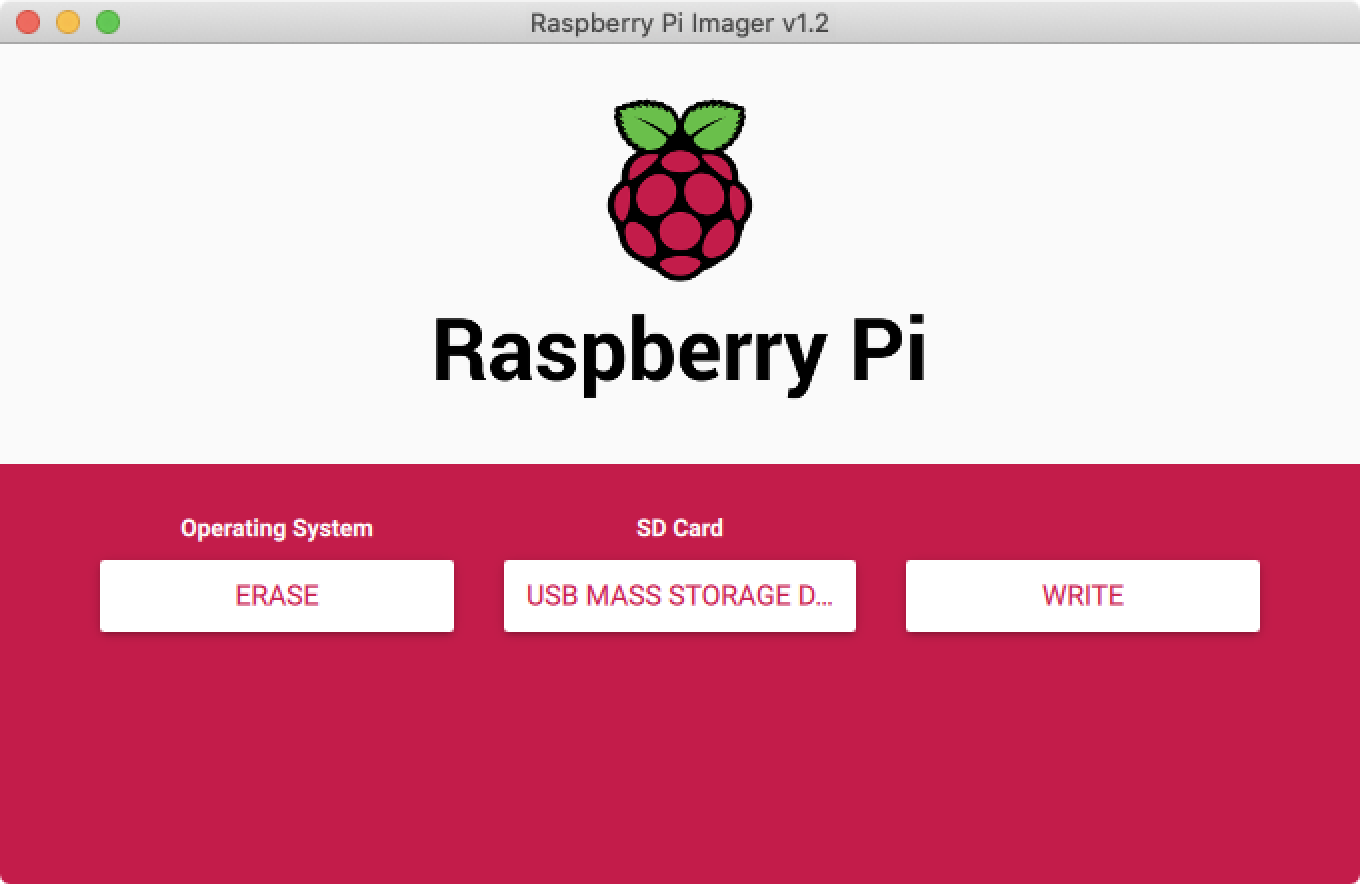
\includegraphics[width=1.0\textwidth]{screenshots/imager-erase.png}
	\caption{Using Raspberry Pi Imager to erase and format a MicroSD card.}
\end{figure}

Then use the Raspberry Pi Imager to write preinstalled server image to the MicroSD card...

\begin{figure}
	\centering	
	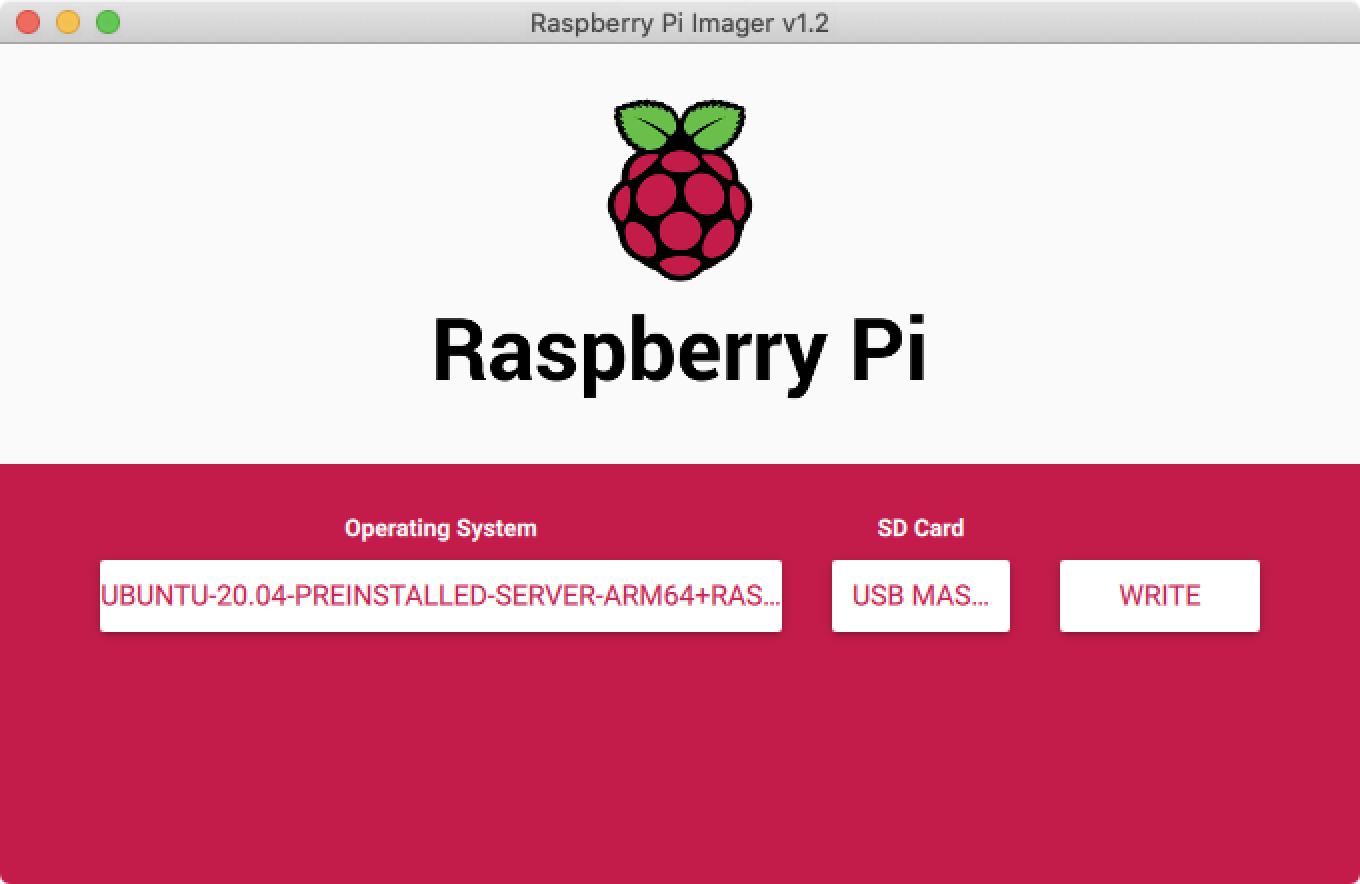
\includegraphics[width=1.0\textwidth]{screenshots/imager-write.png}
	\caption{Using Raspberry Pi Imager to write the server image to a MicroSD card.}
\end{figure}

When complete, remove the MicroSD card from the card reader, place it the Raspberry Pi and plug in the power cable.

The cloud-init configuration process will now start. The Raspberry Pi will acquire its IP address from the router, setup users, update apt, upgrade the system, download software packages, set the hostname (based on the IP address), and finally the system will reboot.


%
% SECTION
%
\clearpage\section{Post-Installation Tasks}

\subsection{Enable No Password Access}

This is required for Open-MPI...

Our public key was installed on each node by cloud-init. So, we can ssh into each node without a password, and use the abbreviated ssh node1, instead of ssh john@node1 (assuming john is the user name on the workstation).

We need to copy our private key to node1 (only node1)...

\lstset{style=type}
\begin{lstlisting}
$ scp ~/.ssh/id_rsa node1:~/.ssh
\end{lstlisting}

Then to enable access to nodes node2 to node9 without a password from node1, we need to import the ... keys into the node1 knownhosts file...

This is easily done. From \verb|macbook|...

\lstset{style=type}
\begin{lstlisting}[]
$ ssh node1
\end{lstlisting}

And then from node1, for \verb|node2| to \verb|node9|...

\lstset{style=type}
\begin{lstlisting}[]
$ ssh node2
\end{lstlisting}

This will generate will generate a message similar to...

\lstset{style=type}
\begin{lstlisting}[]
The authenticity of host 'node2 (192.168.0.2)' can't be established.
ECDSA key fingerprint is SHA256:5VgsnN2nPvpfbJmALh3aJdOeT/NvDXqN8TCreQyNaFA.
Are you sure you want to continue connecting (yes/no/[fingerprint])?
\end{lstlisting}

Respond yes to this, which imports the host key into the \verb|~/.ssh/knownhosts| file of \verb|node1|.

And then exit from the connected node...

\lstset{style=type}
\begin{lstlisting}[]
$ exit
\end{lstlisting}

Repeat the above for \verb|node2| to \verb|node9|.

The above is only required to be done once (unless the host keys on \verb|node2| to \verb|node9| change).


%
% SUB SECTION
%

\subsection{Uninstall unattended-upgrades}

The \verb|unattended-upgrades| package is installed automatically...

This can potentially interferer with long running benchmarks...

Remove...

From \verb|macbook|:

\lstset{style=type}
\begin{lstlisting}[]
$ ssh node1
$ ~/picluster/tools/do "sudo apt remove unattended-upgrades"
\end{lstlisting}

Don't forget to upgrade your cluster regularly at convenient times with...

\lstset{style=type}
\begin{lstlisting}[]
$ ssh node1
$ ~/picluster/tools/upgrade
\end{lstlisting}


\subsection{Add Ubuntu Source Repositories}

We are going to be rebuilding some packages from source...

\lstset{style=type}
\begin{lstlisting}[]
$ ssh node1
$ sudo touch /etc/apt/sources/list.d/picluster.list
$ sudo vim /etc/apt/sources/list.d/picluster.list
\end{lstlisting}

... and add the following source repositories...

\lstset{style=listing}
\begin{lstlisting}[caption=/etc/apt/sources.list.d/picluster.list]
deb-src http://archive.ubuntu.com/ubuntu focal main universe
deb-src http://archive.ubuntu.com/ubuntu focal-updates main universe
\end{lstlisting}

... and then update the repository cache...

\lstset{style=type}
\begin{lstlisting}[]
$ sudo apt update
\end{lstlisting}



\subsection{Create a Project Repository}

Xpand upon...

\lstset{style=type}
\begin{lstlisting}[]
$ ssh node1
$ mkdir picluster
$ cd picluster
$ git init
\end{lstlisting}

Ensure you do push your repository to a remote repository at regular intervals...


\subsection{Select BLAS Library}

The \verb|cloud-init| process will have installed four BLAS libraries, namely...

\verb|libopenblas0-serial|

\verb|libopenblas0-openmp|

\verb|libblis0-serial|

\verb|libblis0-openmp|

To query the BLAS library currently in use on each node we can use one of our Pi Cluster tools...

\lstset{style=type}
\begin{lstlisting}[]
$ ~/picluster/tools/libblas-query
\end{lstlisting}

\lstset{style=type}
\begin{lstlisting}[]
node8... /usr/lib/aarch64-linux-gnu/openblas-openmp/libblas.so.3
node7... /usr/lib/aarch64-linux-gnu/openblas-openmp/libblas.so.3
node6... /usr/lib/aarch64-linux-gnu/openblas-openmp/libblas.so.3
node5... /usr/lib/aarch64-linux-gnu/openblas-openmp/libblas.so.3
node4... /usr/lib/aarch64-linux-gnu/openblas-openmp/libblas.so.3
node3... /usr/lib/aarch64-linux-gnu/openblas-openmp/libblas.so.3
node2... /usr/lib/aarch64-linux-gnu/openblas-openmp/libblas.so.3
node1... /usr/lib/aarch64-linux-gnu/openblas-openmp/libblas.so.3
\end{lstlisting}

To select an alternative library we can use another of our Pi Cluster tools...

\lstset{style=type}
\begin{lstlisting}[]
$ ~/picluster/tools/libblas-set blis-serial
\end{lstlisting}

\lstset{style=type}
\begin{lstlisting}[]
node8... done
node7... done
node6... done 
node5... done 
node4... done 
node3... done 
node2... done 
node1... done 
\end{lstlisting}

\lstset{style=type}
\begin{lstlisting}[]
$ ~/picluster/tools/libblas-query
\end{lstlisting}

\lstset{style=type}
\begin{lstlisting}[]
node8... /usr/lib/aarch64-linux-gnu/blis-serial/libblas.so.3
node7... /usr/lib/aarch64-linux-gnu/blis-serial/libblas.so.3
node6... /usr/lib/aarch64-linux-gnu/blis-serial/libblas.so.3
node5... /usr/lib/aarch64-linux-gnu/blis-serial/libblas.so.3
node4... /usr/lib/aarch64-linux-gnu/blis-serial/libblas.so.3
node3... /usr/lib/aarch64-linux-gnu/blis-serial/libblas.so.3
node2... /usr/lib/aarch64-linux-gnu/blis-serial/libblas.so.3
node1... /usr/lib/aarch64-linux-gnu/blis-serial/libblas.so.3
\end{lstlisting}


%
% CHAPTER
%
\chapter{Install High-Performance Linpack (HPL)}

Download and install the latest version of HPL on \verb|node1|...

\lstset{style=type}
\begin{lstlisting}
$ ssh node1
$ cd ~/picluster
$ mkdir hpl
$ cd hpl
$ wget https://www.netlib.org/benchmark/hpl/hpl-2.3.tar.gz
$ gunzip hpl-2.3.tar.gz
$ tar xvf hpl-2.3.tar
$ rm hpl-2.3.tar
$ cd hpl-2.3
\end{lstlisting}

Create a \verb|Make.picluster| file...

\lstset{style=type}
\begin{lstlisting}
$ cd setup
$ bash make_generic
$ cp Make.UNKNOWN ../Make.picluster
$ cd ..
\end{lstlisting}

Amend \verb|Make.picluster| as per listing ???.

\lstset{style=listing}
\lstinputlisting[caption=~/picluster/hpl/hpl-2.3/Make.picluster]{picluster/hpl/hpl-2.3/Make.picluster}

Build HPL...

\lstset{style=type}
\begin{lstlisting}
$ make arch=picluster   
\end{lstlisting}

This creates the executable \verb|xhpl| and input file \verb|HPL.dat| in \verb|bin/picluster|

The \verb|xhpl| executable has to exist in the same location on each node, so copy \verb|xhpl| to \verb|node2| to \verb|node8| (only \verb|xhpl|, and not \verb|HPL.dat|)...

\lstset{style=type}
\begin{lstlisting}
$ cd bin/picluster
$ ~/picluster/tools/do "mkdir -p picluster/hpl/hpl-2.3/bin/picluster"
$ scp xhpl node2:~picluster/hpl/hpl-2.3/bin/picluster
$ scp xhpl node3:~picluster/hpl/hpl-2.3/bin/picluster
$ scp xhpl node4:~picluster/hpl/hpl-2.3/bin/picluster
$ scp xhpl node5:~picluster/hpl/hpl-2.3/bin/picluster
$ scp xhpl node6:~picluster/hpl/hpl-2.3/bin/picluster
$ scp xhpl node7:~picluster/hpl/hpl-2.3/bin/picluster
$ scp xhpl node8:~picluster/hpl/hpl-2.3/bin/picluster
\end{lstlisting}


%
% CHAPTER
%
\chapter{Install HPC Challenge (HPCC)}

These instructions are derived from the README.txt file in the top level directory of the HPCC source code.

Download and install the latest version of HPCC on \verb|node1|...

\lstset{style=type}
\begin{lstlisting}
$ ssh node1
$ cd ~/picluster
$ mkdir hpcc
$ cd hpcc
$ wget http://icl.cs.utk.edu/projectsfiles/hpcc/download/hpcc-1.5.0.tar.gz
$ gunzip hpcc-1.5.0.tar.gz
$ tar xvf hpcc-1.5.0.tar
$ rm hpcc-1.5.0.tar
$ cd hpcc-1.5.0
\end{lstlisting}

Copy the HPL build script \verb|Make.picluster| to the \verb|hpl| directory...

\lstset{style=type}
\begin{lstlisting}
$ cd hpl
$ cp ~/picluster/hpl/hpl-2.3/Make.picluster .
\end{lstlisting}

Make the following changes to \verb|Make.picluster|. These differ from the build instructions for HPL.

Change the \verb|TOPdir| variable to \verb|../../..|

\lstset{style=hack}
\begin{lstlisting}[caption=Make.picluster]
TOPdir = ../../..
\end{lstlisting}

Add the \verb|math| library explicitly, \verb|-lm|, for the linker...

\lstset{style=hack}
\begin{lstlisting}[caption=Make.picluster]
LAlib = $(LAdir)/libblas.so.3 -lm
\end{lstlisting}

Add the constant \verb|OMPI_OMIT_MPI1_COMPAT_DECLS| to \verb|CCFLAGS|, otherwise the compilation fails...

\lstset{style=hack}
\begin{lstlisting}[caption=Make.picluster]
CCFLAGS = $(HPL_DEFS) -O3 -march=armv8-a -mtune=cortex-a72 -DOMPI_OMIT_MPI1_COMPAT_DECLS
\end{lstlisting}

Now move back up into the top level directory...

\lstset{style=type}
\begin{lstlisting}
$ cd ..
\end{lstlisting}

Build HPCC...

\lstset{style=type}
\begin{lstlisting}
$ make arch=picluster
\end{lstlisting}

Copy the \verb|hpcc| executable to all of the nodes...

\lstset{style=type}
\begin{lstlisting}
$ ~/picluster/tools/do "mkdir -p ~/picluster/hpcc/hpcc-1.5.0"
$ scp hpcc node2:~/picluster/hpcc/hpcc-1.5.0
$ scp hpcc node3:~/picluster/hpcc/hpcc-1.5.0
$ scp hpcc node4:~/picluster/hpcc/hpcc-1.5.0
$ scp hpcc node5:~/picluster/hpcc/hpcc-1.5.0
$ scp hpcc node6:~/picluster/hpcc/hpcc-1.5.0
$ scp hpcc node7:~/picluster/hpcc/hpcc-1.5.0
$ scp hpcc node8:~/picluster/hpcc/hpcc-1.5.0
\end{lstlisting}

Create the input file \verb|hpccinf.txt|...

\lstset{style=type}
\begin{lstlisting}
$ cp _hpccinf.txt hpccinf.txt
\end{lstlisting}

And amend as necessary. An input file which uses 80\% of the total cluster memory is at Listing ???.

To run HPCC across all 8 nodes...

\lstset{style=type}
\begin{lstlisting}
$ mpirun -host node1:4,node2:4,...node7:4,node8:4 -np 32 hpcc
\end{lstlisting}

The output will be in the file \verb|hpccoutf.txt|.




%
% CHAPTER
%
\chapter{Install High Performance Conjugate Gradients (HPCG)}


%
% CHAPTER
%
\chapter{Ubuntu Kernel Build Procedure}

This procedure is derived from the Ubuntu Wiki BuildYourOwnKernel document...

Make sure you have made the source code repositories available as per...

Create a kernel build directory with the correct directory permissions to prevent source download warnings. 

\lstset{style=type}
\begin{lstlisting}
$ ssh node1
$ mkdir -p ~/picluster/build/kernel
$ sudo chown _apt:root ~/picluster/build/kernel
$ cd ~/picluster/build/kernel
\end{lstlisting}

Install the kernel build dependencies...

\lstset{style=type}
\begin{lstlisting}
$ sudo apt-get build-dep linux linux-image-$(uname -r)
\end{lstlisting}

Download the kernel source...

\lstset{style=type}
\begin{lstlisting}
$ sudo apt-get source linux-image-$(uname -r)
$ cd linux-raspi-5.4.0
\end{lstlisting}

This bit is a fix for the subsequent \verb|editconfigs| step of the build procedure...

\lstset{style=type}
\begin{lstlisting}
$ cd debian.raspi/etc
$ sudo cp kernelconfig kernelconfig.original
$ sudo vim kernelconfig
\end{lstlisting}

And make the following change...

\lstset{style=listing}
\begin{lstlisting}[caption=diff kernelconfig kernelconfig.original, numbers=none]
5c5
< 	archs="arm64"
---
> 	archs="armhf arm64"
\end{lstlisting}

Then move back up to the kernel source top level directory...

\lstset{style=type}
\begin{lstlisting}
$ cd ../..
\end{lstlisting}

Prepare the build scripts...

\lstset{style=type}
\begin{lstlisting}
$ sudo chmod a+x debian/rules
$ sudo chmod a+x debian/scripts/*
$ sudo chmod a+x debian/scripts/misc/*
\end{lstlisting}

SOURCE CHANGES AND/OR verb|editconfigs| AT THIS POINT

\lstset{style=type}
\begin{lstlisting}
$ sudo apt install libncurses-dev
$ sudo LANG=C fakeroot debian/rules clean
$ sudo LANG=C fakeroot debian/rules editconfigs
\end{lstlisting}

Tweak the kernel name for identification...

\lstset{style=type}
\begin{lstlisting}
$ cd debian.raspi
$ sudo cp changelog changelog.original
$ sudo vim changelog
\end{lstlisting}

And make the following change, where \verb|+picluster0| is our kernel identifier...

\lstset{style=listing}
\begin{lstlisting}[caption=diff changelog changelog.original, numbers=none]
1c1
< linux-raspi (5.4.0-1015.15+picluster0) focal; urgency=medium
---
> linux-raspi (5.4.0-1015.15) focal; urgency=medium
\end{lstlisting}

Move up to the top level kernel source directory...

\lstset{style=type}
\begin{lstlisting}
$ cd ..
\end{lstlisting}

And build the kernel...

\lstset{style=type}
\begin{lstlisting}
$ sudo LANG=C fakeroot debian/rules clean
$ sudo LANG=C fakeroot debian/rules binary-arch
cd ..
\end{lstlisting}

Install the new kernel...

\lstset{style=type}
\begin{lstlisting}
$ sudo dpkg -i linux*picluster0*.deb
$ sudo shutdown -r now
\end{lstlisting}

Another build procedure fix...

After each kernel build delete the \verb|linux-libc-dev| directory...

\lstset{style=type}
\begin{lstlisting}
$ cd ~/picluster/build/kernel/linux-raspi-5.4.0/debian
$ rm -rf linux-libc-dev
$ cd ..
\end{lstlisting}


%
% CHAPTER
%
\chapter{Build Kernel with No Pre-Emption Scheduler}


%
% CHAPTER
%
\chapter{Build Kernel with Jumbo Frames Support}

Standard MTU is 1500 bytes...

Maximum payload size is 1472 bytes...

NB of 184 (x 8 bytes for Double Precision) = 1472 bytes...

NB $>$ 184 $=>$ packet fragmentation $=>$ reduced network efficiency...

This causes drop of in performance???...

Max MTU on Raspberry Pi 4 Model B is set at build time to 1500...

Not configurable above 1500...

TODO: EXAMPLE OF ERROR MSG...

Need to build the kernel with higher MTU...


Make the required changes to the source... as per REFERENCE

\begin{verbatim}
    cd linux-raspi-5.4.0 

    sudo vim include/linux/if_vlan.h...
        #define VLAN_ETH_DATA_LEN   9000
        #define VLAN_ETH_FRAME_LEN  9018
    
    sudo vim include/uapi/linux/if_ether.h...
        #define ETH_DATA_LEN        9000
        #define ETH_FRAME_LEN       9014
    
    sudo vim drivers/net/ethernet/broadcom/genet/bcmgenet.c...
        #define RX_BUF_LENGTH       10240
\end{verbatim}

Add a Jumbo Frames identifier, "+jf", to the new kernel name...

\begin{verbatim}
    sudo vim debian.raspi/changelog...
        linux (5.4.0-1013.13+jf) focal; urgency=medium
        
\end{verbatim}


%
% CHAPTER
%
\chapter{Rebuild OpenBLAS}

\lstset{style=type}
\begin{lstlisting}
$ ssh node1
$ mkdir -p build/openblas
$ chown -R _apt:root build
$ cd build/openblas
$ sudo apt-get source openblas
$ sudo apt-get build-dep openblas
$ cd openblas-0.3.8+ds
\end{lstlisting}


Edit cpuid\_arm64.c...

\lstset{style=type}
\begin{lstlisting}
$ sudo cp cpuid_arm64.c cpuid_arm64.c.original
$ sudo vim cpuid_arm64.c
\end{lstlisting}


\lstset{style=type}
\begin{lstlisting}
$ diff cpuid_arm64.c cpuid_arm64.c.original
\end{lstlisting}

\lstset{style=type}
\begin{lstlisting}
275c275
<       printf("#define L2_SIZE 1048576\n");
---
>       printf("#define L2_SIZE 524288\n");
278c278
<       printf("#define DTB_DEFAULT_ENTRIES 32\n");
---
>       printf("#define DTB_DEFAULT_ENTRIES 64\n");
\end{lstlisting}


And, then following the instructions in debian/README.Debian

\lstset{style=type}
\begin{lstlisting}
$ DEB_BUILD_OPTIONS=custom dpkg-buildpackage -uc -b
\end{lstlisting}

Once the build is complete..

\lstset{style=type}
\begin{lstlisting}
cd ..
$ sudo apt remove libopenblas0-serial
$ sudo dpkg -i libopenblas0-serial\_0.3.8+ds-1\_arm64.deb
\end{lstlisting}

Ensure the correct BLAS library is being used...

\lstset{style=type}
\begin{lstlisting}
$ sudo update-alternatives --config libblas.so.3-aarch64-linux-gnu
\end{lstlisting}

copy to other nodes
remove old...
install new...

If more than one BLAS library is installed, check update-alternatives!!!

ssh node2 .. node8
\lstset{style=type}
\begin{lstlisting}
$ ssh node2 sudo apt remove libblas0-serial
$ scp libopenblas0-serial\_0.3.8+ds-1\_arm64.deb node2:~
$ ssh sudo dpkg -i libopenblas0-serial\_0.3.8+ds-1\_arm64.deb
$ ssh sudo update-alternatives --config libblas.so.3-aarch64-linux-gnu
\end{lstlisting}


%
% CHAPTER
%
\chapter{Rebuild BLIS}

\lstset{style=type}
\begin{lstlisting}
$ ssh node1
$ mkdir -p picluster/build/blis
$ cd picluster/build/blis
$ apt-get source blis
$ sudo apt-get build-dep blis
$ cd blis-0.6.1
\end{lstlisting}


%
% CHAPTER
%

\chapter{Build OpenMPI from Source}

Do all of this on node1...

\lstset{style=type}
\begin{lstlisting}
$ ssh node1
\end{lstlisting}

We want to avoid collisions with multiple OpenMPI installations, so remove original installed version...

\lstset{style=type}
\begin{lstlisting}
$ sudo apt remove openmpi-common
$ sudo apt remove openmpi-bin
$ sudo apt autoremove 
\end{lstlisting}

OpenMPI requires the libevent-dev package...

\lstset{style=type}
\begin{lstlisting}
$ sudo apt install libevent-dev
\end{lstlisting}

Create a build directory, and download and, and and following BLAH, BLAH build OpenMPI...

\lstset{style=type}
\begin{lstlisting}
$ mkdir -p ~/picluster/build/openmpi
$ cd ~/picluster/build/openmpi
$ wget https://download.open-mpi.org/release/open-mpi/v4.0/openmpi-4.0.4.tar.gz
$ gunzip openmpi-4.0.4.tar.gz
$ tar xvf openmpi-4.0.4.tar
$ rm openmpi-4.0.4.tar
$ cd openmpi-4.0.4
$ mkdir build
$ cd build
$ ../configure CFLAGS="-O3 -march=armv8-a -mtune=cortex=a72"
$ make all
$ sudo make install
$ sudo ldconfig
\end{lstlisting}

OpenMPI will installed to /usr/local

EXTRACT FROM HPL.dat


TODO: HOW TO COPY TO ALL NODES!


%
% CHAPTER
%
\chapter{Aerin Cluster Tools}

\lstinputlisting[caption=picluster/tools/upgrade, numbers=left, backgroundcolor=\color{LightSkyBlue}]{picluster/tools/upgrade}
\lstinputlisting[caption=picluster/tools/reboot, numbers=left, backgroundcolor=\color{LightSkyBlue}]{picluster/tools/reboot}
\lstinputlisting[caption=picluster/tools/shutdown, numbers=left, backgroundcolor=\color{LightSkyBlue}]{picluster/tools/shutdown}
\lstinputlisting[caption=picluster/tools/libblas-query, numbers=left, backgroundcolor=\color{LightSkyBlue}]{picluster/tools/libblas-query}
\lstinputlisting[caption=picluster/tools/libblas-set, numbers=left, backgroundcolor=\color{LightSkyBlue}]{picluster/tools/libblas-set}


%
% CHAPTER
%

\chapter{Arm Performance Libraries}

\textcolor{red}{This does not work, yet! HPL will compile and link to Arm Performance Libraries, but raises an illegal instruction error at runtime.}

\textcolor{red}{At the time of writing, Arm Performance Libraries release 20.2.0 requires a minimum Instruction Set Architecture (ISA) of armv8.1-a. Unfortunately, the Raspberry Pi's Cortex-A72 ISA is armv8.0-a. An Arm representative has indicated on the Arm HPC Forum that the next release of the libraries will support the armv8.0-a ISA.}

\textcolor{red}{This Chapter is included for future reference.}

The Arm Performance Libraries website states:

"Arm Performance Libraries provides optimised standard core math libraries for high-performance computing applications on Arm processors. This free version of the libraries provides optimised libraries for Arm® Neoverse™ N1-based Armv8 AArch64 implementations that are compatible with various versions of GCC. You do not require a license for this version of the libraries."

To install Arm Performance Libraries, firstly downloaded Arm Performance Libraries 20.2.0 with GCC 9.3 for Ubuntu 16.04+ from the Arm website.

Then follow these instructions.

\lstset{style=type}
\begin{lstlisting}
$ ssh node1
\end{lstlisting}

Install the required \verb|environment_modules| package.

\lstset{style=type}
\begin{lstlisting}
$ sudo apt install environment-modules
\end{lstlisting}

Then extract and install Arm Performance Libraries.

The default installation directory is /opt/arm.

\lstset{style=type}
\begin{lstlisting}
$ mkdir ~/picluster/armpl
$ cd ~/picluster/armpl
$ tar xvf arm-performance-libraries_20.2_Ubuntu-16.04_gcc-9.3.tar
$ rm arm-performance-libraries_20.2_Ubuntu-16.04_gcc-9.3.tar
$ sudo ./arm-performance-libraries_20.2_Ubuntu-16.04.sh
\end{lstlisting}

Copy the \verb|Make.picluster| configuration file.

\lstset{style=type}
\begin{lstlisting}
$ cd ~/picluster/hpl/hpl-2.3
$ cp Make.picluster Make.picluster-armpl
\end{lstlisting}

Make the following changes to \verb|Make.picluster-armpl|.

\lstset{style=listing}
\begin{lstlisting}[caption=Make.picluster-armpl, numbers=none]
LAdir        = /opt/arm/armpl_20.2_gcc-9.3
LAinc        =
LAlib        = -L$(LAdir)/lib -larmpl -lgfortran -lamath -lm
\end{lstlisting}

Build HPL.

\lstset{style=type}
\begin{lstlisting}
$ make arch=picluster-armpl
\end{lstlisting}


%
% THE END
%
\end{document}
